\chapter{M-dwarf selection through near-infrared photometry}
\label{ChapPhot}
\footnote{The contents of this chapter were originally published in the Monthly Notices of the Royal Astronomical Society \citep{2019Bentley}.}
As they are the most common main-sequence dwarf in the galaxy, M-dwarfs are the best candidates for habitable zone exoplanets. However the M-dwarfs need to be identified. Due to the limited amount of time available on high precision spectroscopes, and the rate at which spectra can be obtained, classifying stars one at a time is not efficient. Recent improvements in technology have allowed for the consideration of multi-star, spectroscopic surveys which can obtain spectra in bulk, leading to the classification of thousands of stars per night. LAMOST is one example of these types of surveys (see Section \ref{secSpecSurveys} for details).\\

While this means spectra can be obtained for a large number of stars and identify the M-dwarfs within the selection, an initial selection criteria is still required. Ideally, a sample of likely M-dwarfs would be selected, using either astrometric or photometric information, then classifying this sample to determine the M-dwarfs present.\\

The use of proper motion selection has dominated M-dwarf identification to date (e.g. \citealt{1979Luyten}; \citealt{2000Zacharias}), with the reduced proper motion H; \citep{1922Luyten} being used to identify stars likely to be close to the Sun (and therefore low in luminosity). This does have the disadvantage, however, of only probing two components of each star's three-dimensional space motion, and so necessarily produces a biased sample.\\

Selecting a purely distance- and luminosity-limited sample, through absolute magnitude, has always been the ultimate goal of M-dwarf selection, but has been impossible until recently due to the absence of all-sky, magnitude-limited astrometric surveys. However, with the release of {\em Gaia} DR2 \citep{2016Gaia}, and the forthcoming releases of even more complete surveys from DR3 onwards, such a sample selection for M-dwarfs is now becoming possible.\\

Photometric colour based M-dwarf selection suffers from contamination by non-M-dwarfs due to photometric uncertainties in the apparent magnitudes, source contamination and the intrinsic scatter of stellar properties about any adopted relationships between observed colours and physical parameters. On the other hand, they do not suffer kinematic biases, and there are now very large, high-quality and publicly available all-sky databases at the optical and near-infrared wavelengths best suited to M-dwarf selection. The combination of the all-sky, magnitude-limited distances from {\em Gaia} DR2, and the availability of large, deep and all-sky multi-colour surveys like 2MASS and WISE (see Section\,\ref{secTransitSurveys}) means we are now in an era when both luminosity-selection and photometric-selection can deliver kinematically unbiased large samples of M-dwarfs suitable for follow-up spectroscopic confirmation.\\

This work intended to develop the criteria by which a sample of probable M-dwarfs can be identified, using photometry and distance, to then be confirmed by the FunnelWeb survey. The FunnelWeb survey has been cancelled but this method is applicable to any multi-star spectroscopic survey.
\section{Data}
\subsection{Survey data}
\label{secObsData}
As it is the most comprehensive survey of luminosity and distance currently available, the primary data set is comprised from {\em Gaia}. It was decided to use the {\em Gaia} G band exclusively over the R and B passbands as G is derived directly from the blue and red {\em Gaia} passbands, and the short wavelength range between B and R give very little unique colour information at the wavelengths required for studying M-dwarfs. In addition, the WISE and 2MASS all-sky surveys provide photometry at a range of optical and near-infrared wavelengths. In particular, as can be seen from Figure\,\ref{figPassband}, they probe critical wavelengths for the selection of M-dwarfs, which emit most of their flux between 0.6\,nm and 5\,$\mu$m. As such, the observational dataset includes apparent magnitudes from {\em Gaia}, WISE, and 2MASS. \\

\begin{figure}
    \centering
    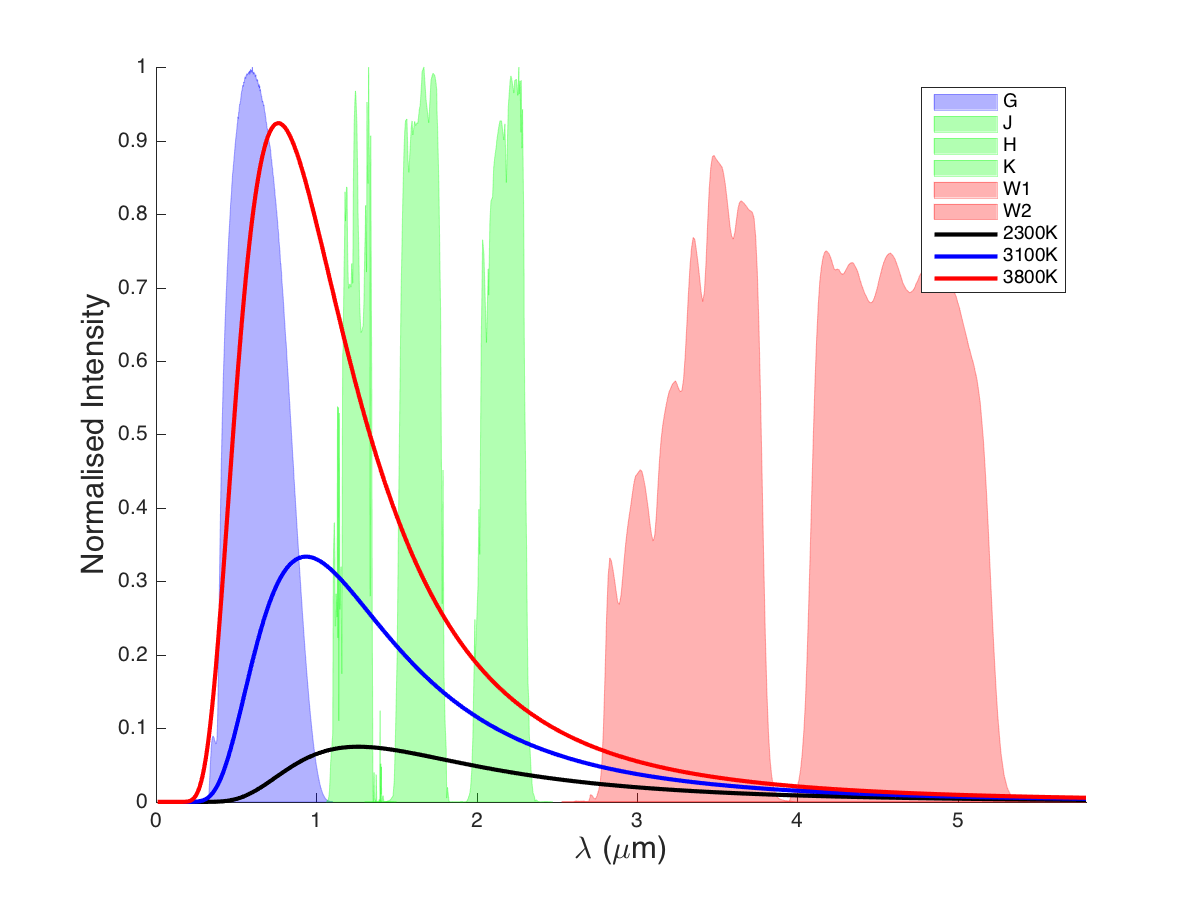
\includegraphics[width=0.8\textwidth]{Passbands.png}
    \caption{The wavelength coverage of the Gaia, 2MASS, and WISE photometry passbands. Overplotted is the blackbody curves of a M0 (red), M4 (blue) and M9 (black) star.}
    \label{figPassband}
\end{figure}

Using the {\em Gaia} archive\footnote{http://gea.esac.esa.int/archive/}, a working dataset of all objects from {\em Gaia} DR2 \citep{2018GaiaDR2} with G\,$<$\,14.5 was selected. These objects were also cross-matched against the 2MASS PSC and {\em WISE} AllWISE catalogues using their respective ``best neighbour'' cross match tables which use position and proper motion to match external catalogues to {\em Gaia} (see \citealt{2017Marrese} for full details). Additionally, the area of sky selected was limited to that accessible from the southern hemisphere ($\delta$\,\textless\,+10\,\degree) and avoided the Galactic plane ($|$b$|>$10\,\degree) -- the latter criterion was adopted because the large WISE full-width-at-half-maximum ($\approx$\,6\,") makes it difficult to match, or rely on, its data in crowded fields. Any object flagged in the AllWISE catalogue as a galaxy (xscproc\,$\neq$\,null), an extended object (ext\_flg\,$\neq$\,0), as multiple objects (n\_2mass\,\textgreater\,1) or as objects with poor/contaminated photometry (cc\_flags\,$\neq$\,0000) was also removed. The resulting catalogue contains roughly 8 million stars at G\,\textless\,14.5. Of these 8 million stars, 107,743 have no 2MASS cross-match and 627,127 have no WISE cross-match. For each star, photometry was required from all three surveys. Due to this, 638,845 stars were removed due to lack of cross-matches. This means that of all the observable stars with the requirements mentioned above, roughly 8\% will be missing from the sample.
\subsection{Spectroscopic comparison sample}
\label{secSpecData}
To provide a comparison set of photometry for stars with known spectral classifications, the same Gaia, 2MASS and WISE photometry was extracted for the large sample of M-dwarfs spectrally classified by \cite{2011West}, supplemented by the late K-dwarfs classified by \cite{2015Zhong}\footnote{While the Zhong K-dwarfs were useful for investigating the colour space where the K- and M-dwarfs intersect, the K7.5 stars were not included when determining the colour-subtype relationships (although their median colour values were included in Table 2.1 for completeness). The classification scheme used by \citealt{2015Zhong} is not the usual  Morgan–Keenan (MK) system, but is instead adapted from \citealt{2003Lepine}. While the K7 stars are classified using the Lepine system, their spectra should not differ significantly from the MK K7 spectral standard of 61 Cygni B and it is reasonable to include them in the analysis. The MK system does not recognise a K7.5 subtype and so they needed to be excluded.} This comparison sample consisted only of the stars that were quiescent for the passbands used in this work (var\_flg = XX\_\_, where X is from 0-5), and if the uncertainty in the {\em Gaia} parallax was less than, or equal to, 5\% of the parallax ($\sigma_\varpi/\varpi \leq 0.05$). Otherwise this comparison sample was selected in the same manner as the main sample. It should be noted that 99\% of these stars are dimmer than the G\,$<$\,14.5 magnitude limit of the main sample, however 54\% are within 229 pc, the magnitude limiting distance for observing M-dwarfs at G\,$<$\,14.5 (see Section\,\ref{secCombined}) and the photometric uncertainty was required to be 5\% or less of the magnitude. As such, the sample was not magnitude limited.\\

\begin{figure*}
	\centering
    \subfloat[]{\label{figRelGJ}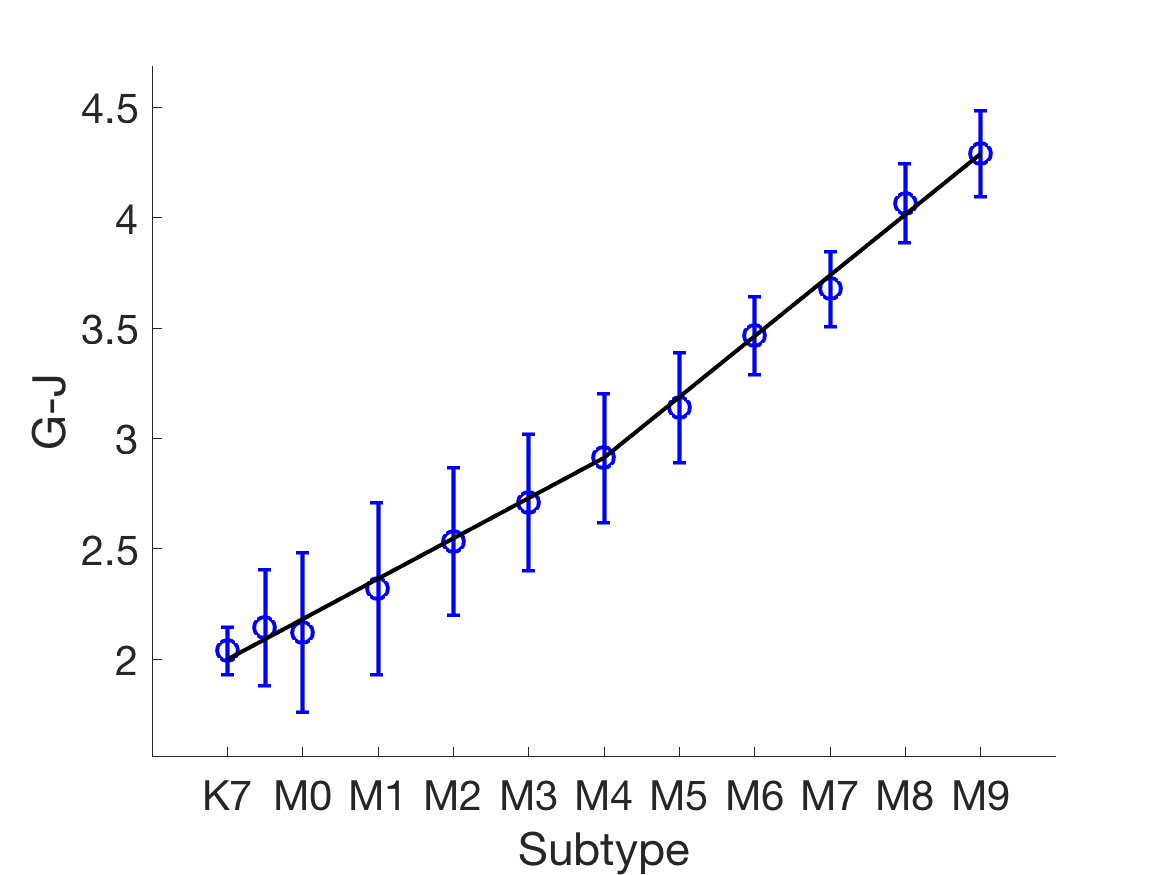
\includegraphics[width=0.5\textwidth]{RelationshipGJ.png}}
    \subfloat[]{\label{figRelGK}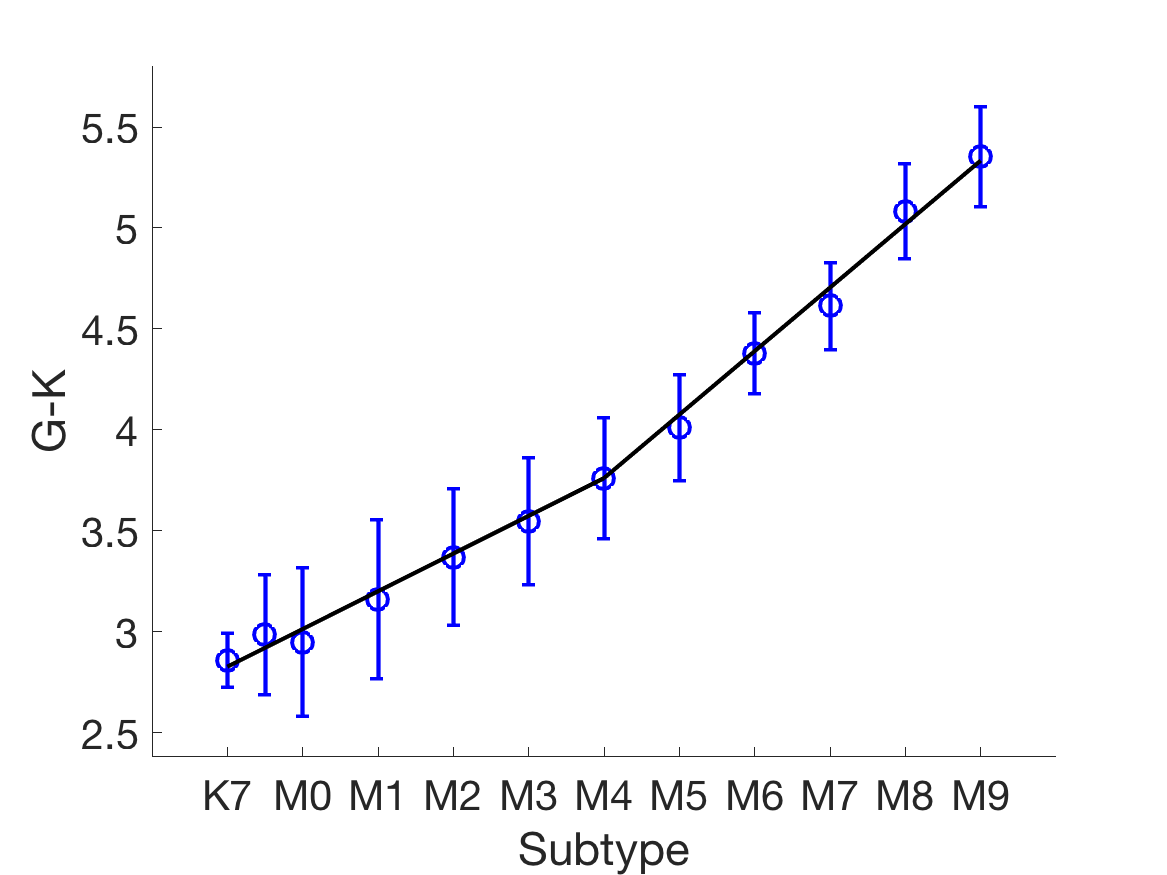
\includegraphics[width=0.5\textwidth]{RelationshipGK.png}}\\
    \subfloat[]{\label{figRelKW2}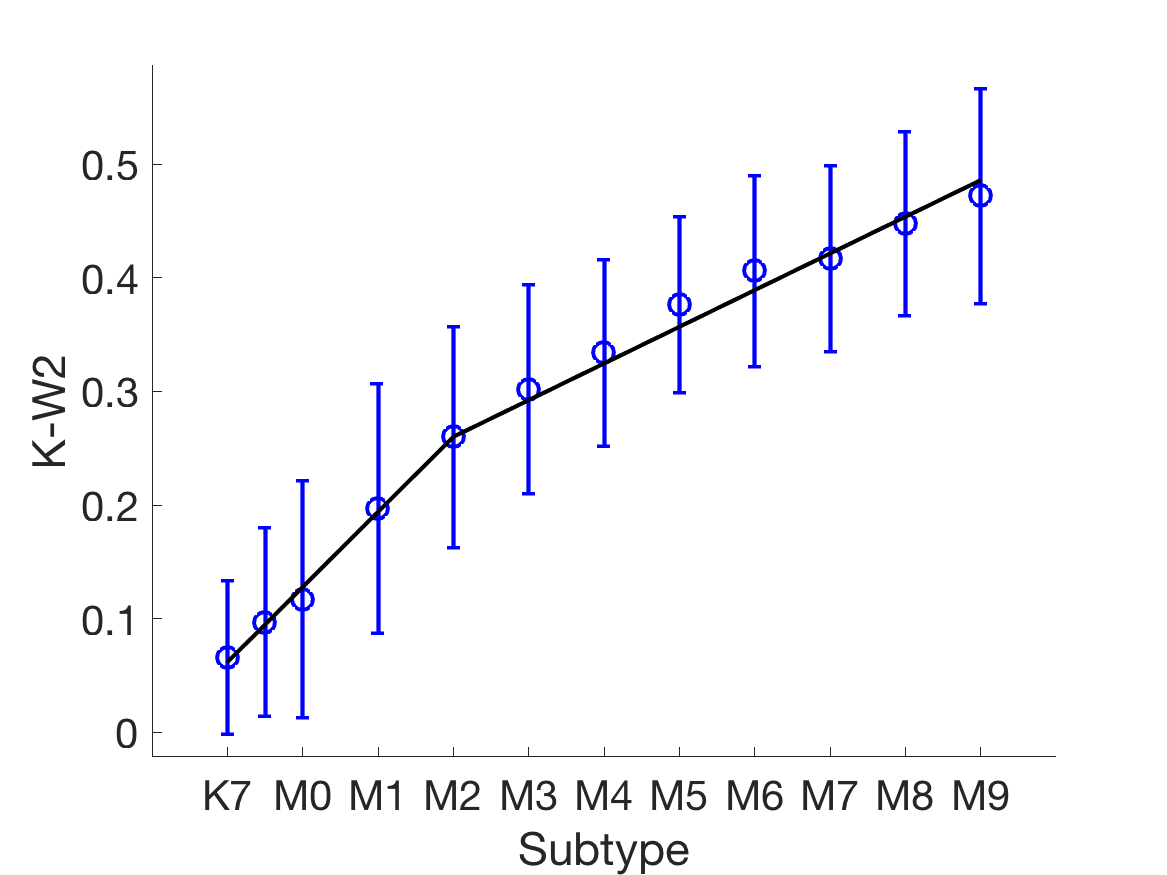
\includegraphics[width=0.5\textwidth]{RelationshipKW2.png}}
    \subfloat[]{\label{figRelW1W2}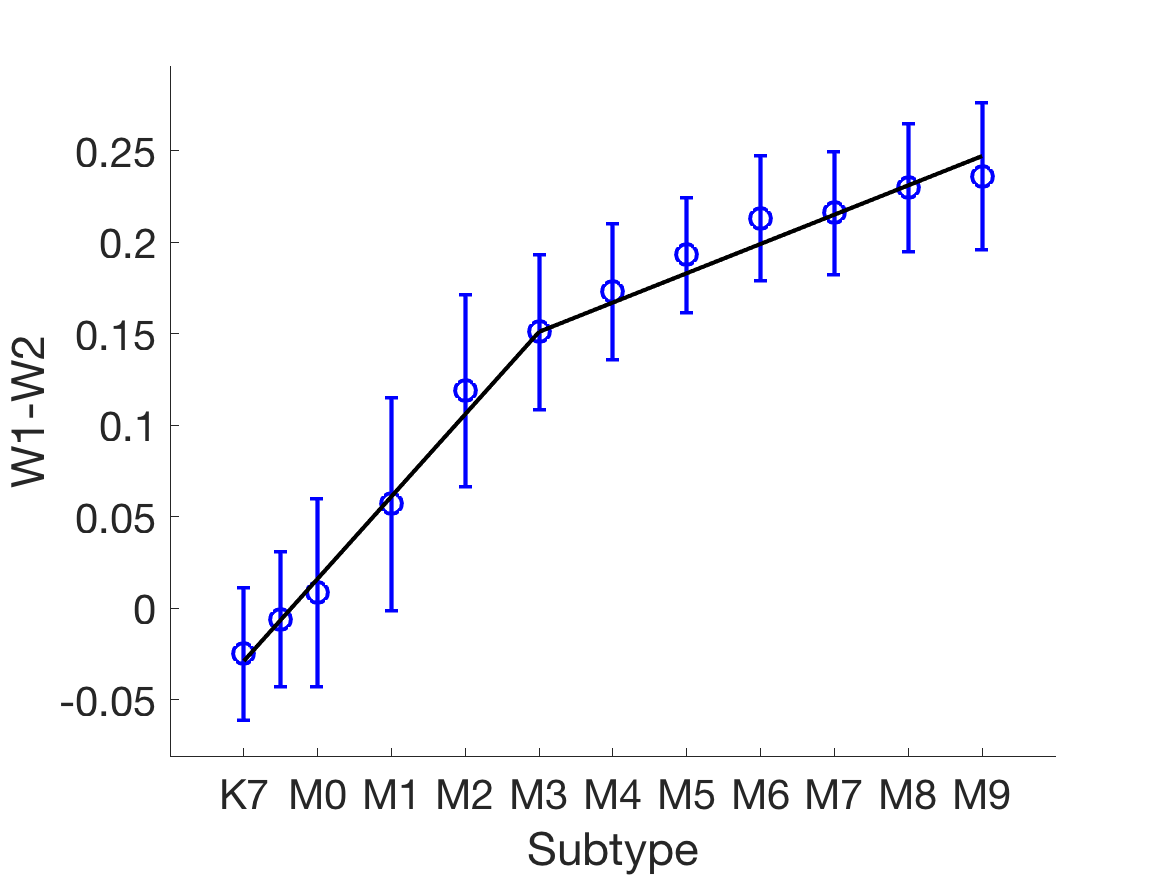
\includegraphics[width=0.5\textwidth]{RelationshipW1W2.png}}\\
    \subfloat[]{\label{figRelJK}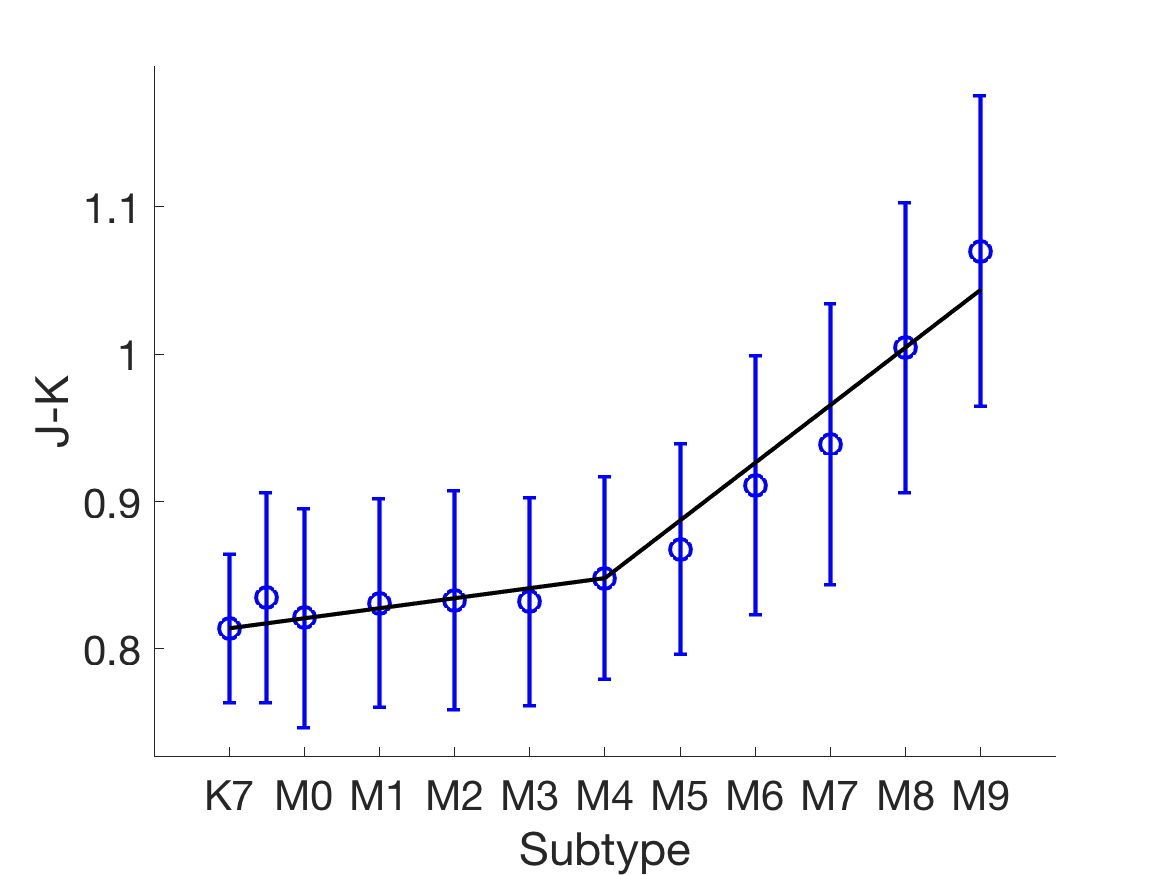
\includegraphics[width=0.5\textwidth]{RelationshipJK.png}}
    \caption{Photometric Gaia/2MASS/WISE colours as a function of spectral type for M-dwarfs of West et al. (2011) and late K-dwarfs of Zhong et al. (2015). Circles are the median colour values for each subtype, with uncertainty bars showing r.m.s scatter. The solid black lines are linear fits to the median subtypes. The outlier K7.5 median colour value for J--K was excluded when determining that parameterisation.}
	\label{FigRelationship}
\end{figure*}

Median colours were calculated and the r.m.s. scatter about the mean for each \citealt{2011West} defined spectral type, along with linear parametrisations of the median colours. The results of these parametrisations can be seen in Figure\,\ref{FigRelationship} for multiple colours and are tabulated in Table\,\ref{TabLookup} as a function of spectral type. In general the photometric scatter around these linear relationships are large - usually several tenths of a magnitude - with the scatter for optical-infrared colours becoming as large as seven-tenths of a magnitude at early types. This is much larger than expected due to the photometric measurement uncertainty of these surveys, suggesting this scatter is dominated by cosmic scatter due to metallicity variations, age variations, unresolved binarity, etc. Nonetheless, the trends with spectral type are consistent and smoothly varying\footnote{From the figures, it is clear that the parameterisation for each colour is represented by two linear relationships. The slope of the relationships, and the subtype at which one relationship changes to the second, varies with colour. Unlike the majority of the colours where the rate of change in colour increases with later subtypes, those with one, or both, of the WISE passbands display a lower rate of change. This may be due to the lower levels of flux across the WISE bands (see Figure\,\ref{figPassband}).} Figure\,\ref{figSubtypes} shows the spectral type distribution for J--W1/W1--W2, overplotted on a synthetic population (see Section\,\ref{secModel}).

\begin{table*}
	\begin{tabular}{| l | c | c  c | c c | c c | c c | l |}
	\hline
	Type & N  & G--J & r.m.s. & G--K & r.m.s. & K--W2 & r.m.s. & W1--W2 & r.m.s. & Src\\
	\hline
	K7 & 211 & 1.999 & 0.302 & 2.826 & 0.309 & 0.062 & 0.09 & -0.029 & 0.046 & ZJ \\
	K7.5 & 153 & 2.091 & 0.296 & 2.92 & 0.305 & 0.095 & 0.09 & -0.006 & 0.046 & ZJ \\
	M0 & 1160 & 2.182 & 0.291 & 3.013 & 0.302 & 0.128 & 0.09 & 0.016 & 0.045 & WA \\
	M1 & 1127 & 2.364 & 0.28 & 3.2 & 0.294 & 0.194 & 0.089 & 0.061 & 0.044 & WA \\
	M2 & 1999 & 2.547 & 0.269 & 3.387 & 0.287 & 0.26 & 0.089 & 0.106 & 0.043 & WA \\
	M3 & 2948 & 2.73 & 0.259 & 3.574 & 0.28 & 0.292 & 0.088 & 0.151 & 0.042 & WA \\
	M4 & 2608 & 2.912 & 0.248 & 3.761 & 0.273 & 0.325 & 0.088 & 0.167 & 0.04 & WA \\
	M5 & 1162 & 3.188 & 0.237 & 4.075 & 0.266 & 0.357 & 0.087 & 0.183 & 0.039 & WA \\
	M6 & 1355 & 3.463 & 0.227 & 4.39 & 0.259 & 0.389 & 0.087 & 0.199 & 0.038 & WA \\
	M7 & 1240 & 3.739 & 0.216 & 4.705 & 0.251 & 0.421 & 0.086 & 0.215 & 0.037 & WA \\
	M8 & 418 & 4.014 & 0.205 & 5.019 & 0.244 & 0.454 & 0.086 & 0.231 & 0.036 & WA \\
    M9 & 231 & 4.29 & 0.195 & 5.334 & 0.237 & 0.486 & 0.085 & 0.247 & 0.034 & WA \\
	\hline
	\end{tabular}
    \caption{Colour sequences (and r.m.s. scatter about them) for late-K- and M-dwarfs. Spectral type sources are: ZJ, Zhong et al. (2015); WA, West et al. (2011).}
    \label{TabLookup}
\end{table*}
\section{Simulations}
\label{secModel}
To test colour-based selection criteria,  simulated photometry of a synthetic population of stars was created using {\em Galaxia} \citep{2011Sharma}. This is a Galactic simulation code that generates a synthetic stellar population, including parameters for every star simulated such as their masses, ages, temperatures and simulated photometry. {\em Galaxia} generates its synthetic populations based on models for the Galaxy's stellar populations and its star formation history. It first generates a population with a set of basic physical parameters (position, distance, mass, age, metallicity) very similar to the Besan\c{c}on model \citep{2003Robin}  to generate the thin disc, the thick disc, the bulge and the halo populations (respectively). It then derives the resulting luminosity, effective temperature, photometric magnitudes and colours for each star, using the PARSEC-v1.2S isochrones \citep{2012Bressan, 2014Tang, 2014Chen, 2015Chen}, the NBC version of bolometric corrections \citep{2014Chen}, and assuming Reimers mass loss with efficiency $\eta=0.2$ for RGB stars. This photometry then has corrections applied to simulate the effects of extinction \citep{2011Sharma}. These simulations therefore include the effects of cosmic scatter due to metallicity variation and extinction, but do not include photometric measurement scatter, or the effects of source confusion. The simulation generated for this work was initially created for a magnitude limit of G\,\textless\,16, so that it would remain complete to G\,=\,14.5 when subject to the impacts of extinction and photometric scatter.\\

Because the {\em Galaxia} population is generated based on physical parameters,  relationships between those parameters (i.e. mass, radius, gravity, age, temperature) and the predicted spectral types of interest needed to be determined. In particular, what gravities and effective temperatures correspond to M-dwarfs? The temperature and gravity estimates of Table 4.1 from \citet{2005Reid} were adopted in this work -- specifically a {\em Galaxia} object is considered an M-dwarf if it has 2250\,K\,\textless\,T\,\textless\,3900\,K and 4.2\,\textless\,$\log g$\,\textless\,5.4. Any object younger than 500\,Myr was not considered an M-dwarf for this work. This, plus estimates for K-dwarfs, M- and K-giants, are presented in Table\,\ref{TabMK}. The M-dwarf classification identifies $\approx$\,20,000 stars as M-dwarfs within the G\,\textless\,14.5 {\em Galaxia} sample of $\approx$\,4.9 million stars.\\

\begin{table}
\begin{center}
	\begin{tabular}{| c | c | c | c |}
		\hline
        Sp. Type & log(g) & Age\,(Yr) & T\,(K) \\
        \hline
        M-dwarf & 4.2\,-\,5.4 & \textgreater\,5\,x\,10$^{8}$ & 2250\,-\,3900 \\
        K-dwarf & 4.2\,-\,5.4 & \textgreater\,5\,x\,10$^{8}$ & 3900\,-\,4600 \\
        M-giant & \textless\,4.2 & \textgreater\,5\,x\,10$^{8}$ & 2250\,-\,3900 \\
        K-giant & \textless\,4.2 & \textgreater\,5\,x\,10$^{8}$ & 3900\,-\,4600 \\
        \hline
\end{tabular}
\caption{Stellar characteristics used to define the M and K, dwarf and giant populations in the synthetic {\em Galaxia} population.}
\label{TabMK}
\end{center}
\end{table}
Figure\,\ref{figScatterB} shows a density plot of this {\em Galaxia} sample in the J--W1/W1-W2 plane, along with the objects identified as M-dwarfs by the adopted criterion (over-plotted in red).\\

{\em Galaxia} is necessarily limited in its predictive power for the photometry of sources by its PARSEC stellar models. In particular, {\em Galaxia} cannot predict the photometric properties of the latest M-dwarfs, because they are not included in the PARSEC isochrones. Specifically there are no isochrones for dwarfs of later than M5 (i.e. for T\,\textless\,2700\,K with 4.2 $<$ $\log g$ $<$ 5.4). This is highlighted in Figure\,\ref{figSubtypes} an expanded region of Figure \ref{figScatterB} around the M-dwarf branch, along with the M-dwarf sequence for spectroscopically observed M-dwarfs from Section\,\ref{secSpecData}. The latest spectroscopically observed M-dwarfs (M6-9 plotted in blue) lie in a region where {\em Galaxia} simulates almost no objects, because it {\em can} simulate no objects.\\

\begin{figure}[!ht]
    \centering
    \subfloat[]{\label{figScatterA}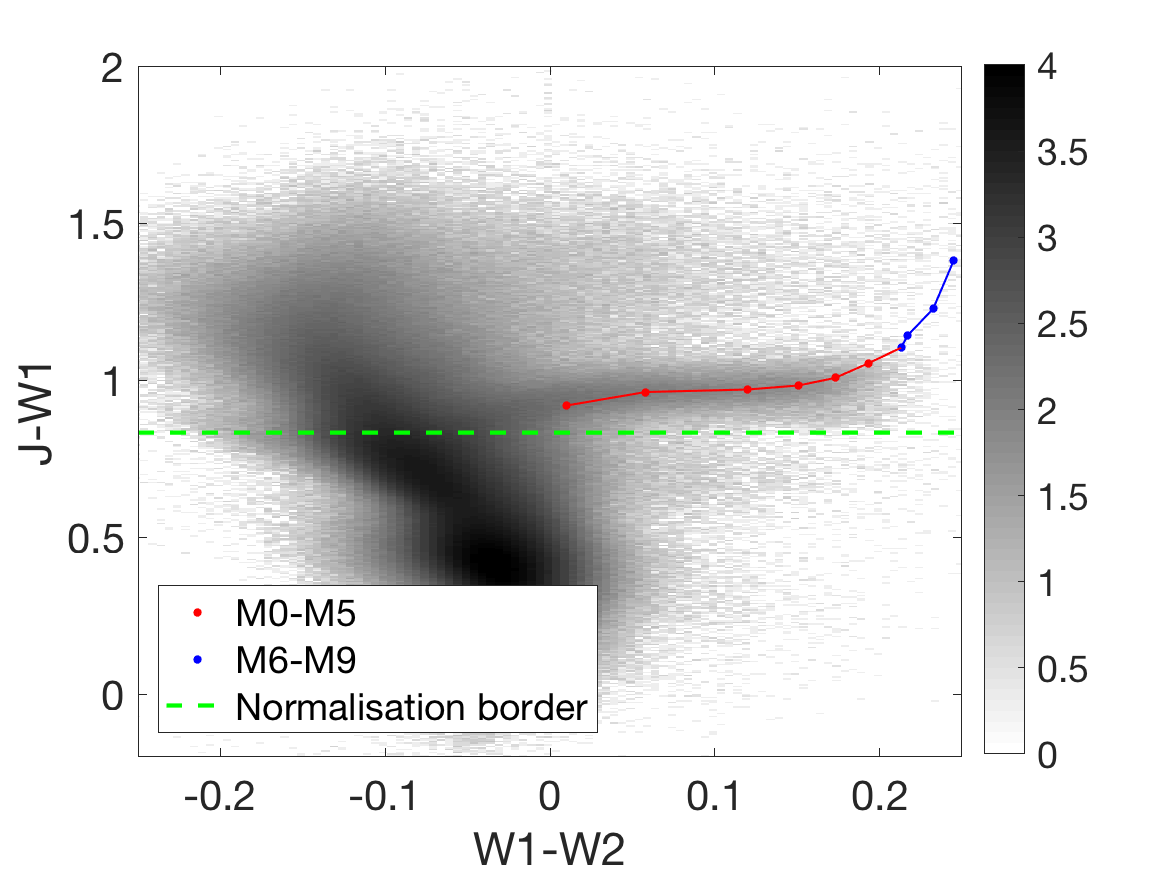
\includegraphics[width=0.8\textwidth]{MDwise.png}}\\
    \subfloat[]{\label{figScatterB}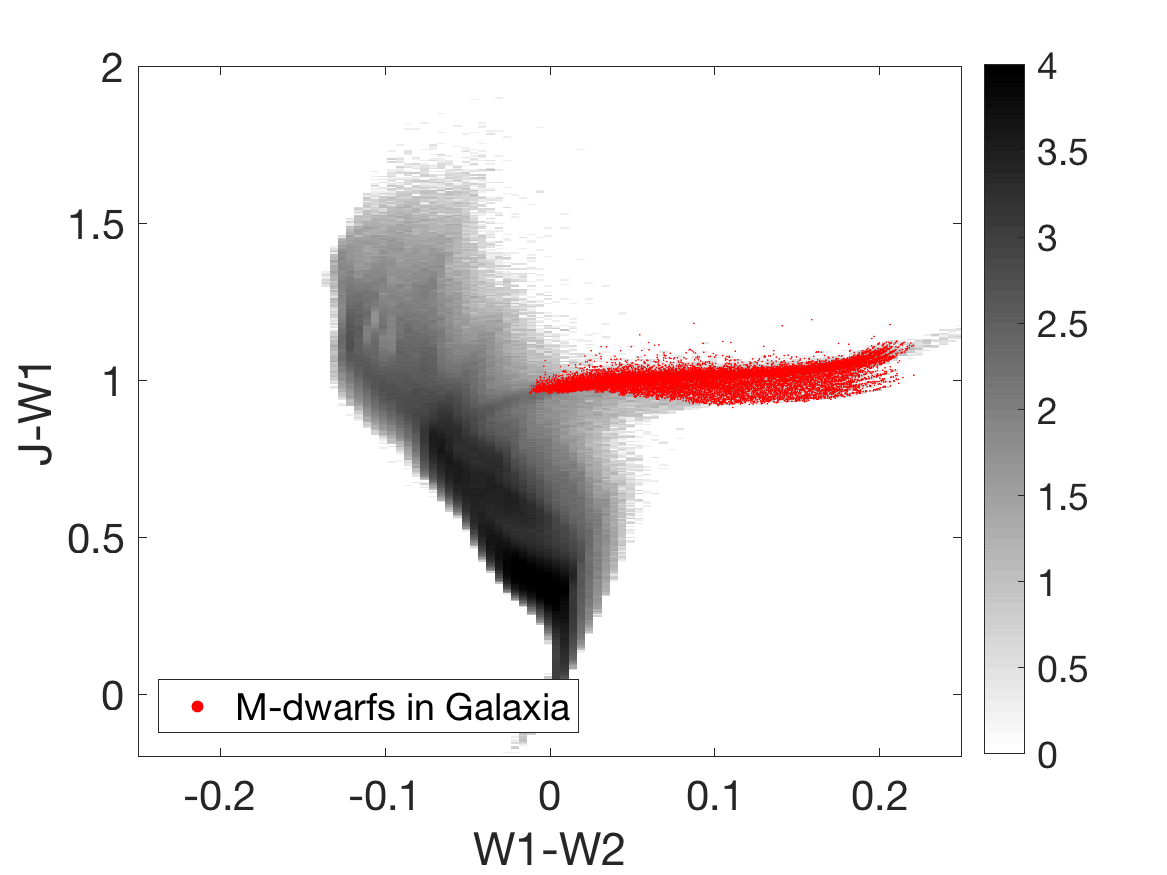
\includegraphics[width=0.8\textwidth]{MDgalaxia.png}}
    \caption{Logarithmic source densities in the J--W1/W1--W2 plane for sources with 9\,\textless\,G\,\textless\,14.5. Figure\,\ref{figScatterA} shows the {\em Gaia}/WISE/2MASS data. Objects below the green horizontal line in the  are used to normalise {\em Galaxia} to observational data, and the M-dwarf spectroscopic comparison sample from Section\,\ref{secSpecData} are overplotted in red and blue. Figure\,\ref{figScatterB} shows the {\em Galaxia} synthetic star population including cosmic scatter and extinction, but without photometric measurement scattering. M-dwarfs (see text) are highlighted in red.} 
    \label{figScatter}
\end{figure}
However, it should be noted that:
\begin{itemize}
	\item The number of M dwarfs will drop dramatically at later spectral types in any magnitude limited sample.
	\item These late M-dwarfs have photometric properties that are well-known from other work \citep{2002Leggett} and Section\,\ref{secSpecData} making them quite easy to distinguish from M-giants and other types of stars\,\citep{2011Lepine}.
	\item The TESS survey (at least) will focus on M-dwarfs earlier than M5 \citep{2015Ricker}.
\end{itemize}
As a result these ``missing'' {\em Galaxia} late M-dwarfs will make an insignificant contribution to estimates of completeness and contamination.\\

\begin{figure}[!ht]
	\centering
	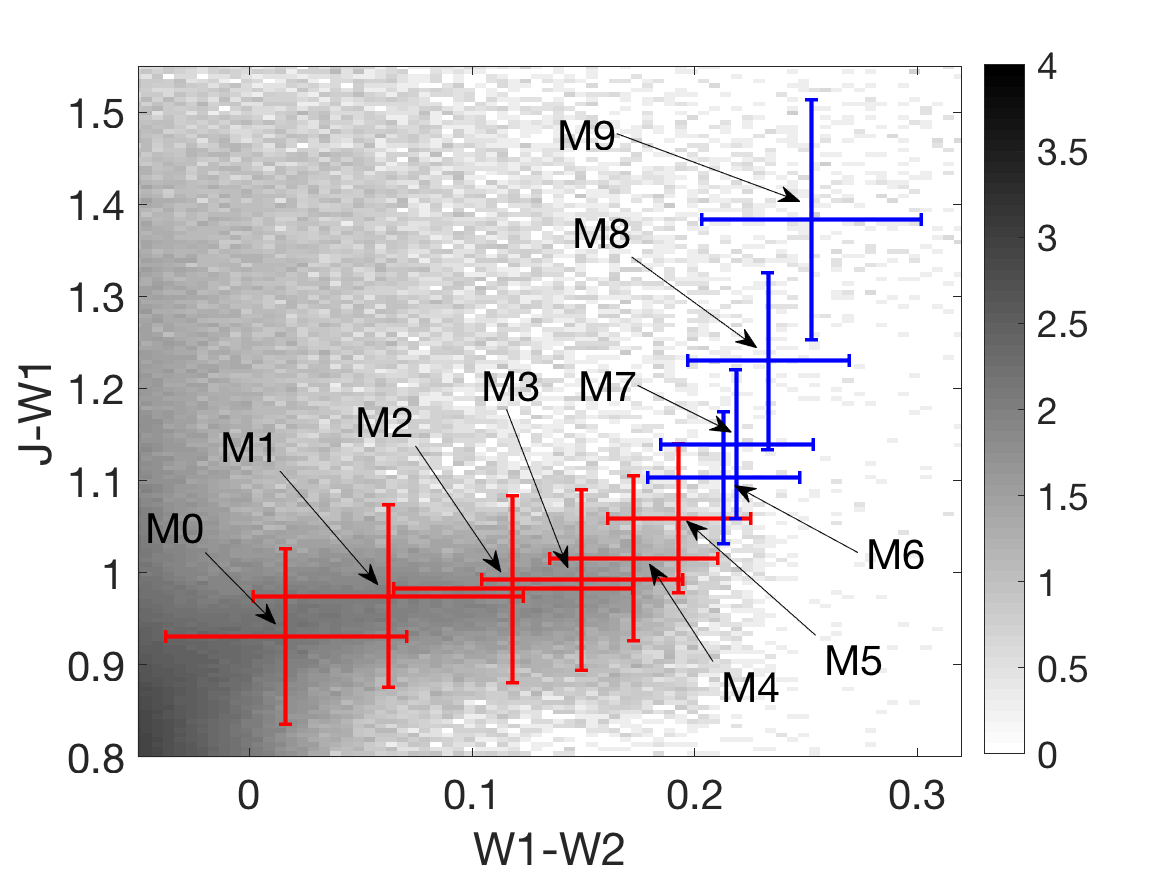
\includegraphics[width=0.8\textwidth]{Subtypes-2.png}
    \caption{{\em Galaxia} generated colour-colour density in J--W1/W1--W2 expanded around the M-dwarf branch. Overplotted are points representing the median colour and r.m.s. for spectroscopically observed M-dwarfs (M0-M5 in red, M6-M9 in blue).}
    \label{figSubtypes}
\end{figure}
\subsection{Photometric scatter}
\label{Scattering}
As noted above, scatter needs to be added to  {\em Galaxia}'s simulated photometry to match the expected photometric uncertainties for the observational data -- this is obvious from Figs. \ref{figScatterA} and \ref{figScatterB}, where it can be seen that the observed distribution is noticeably more scattered from the {\em Galaxia} one.\\

The observational data all come with estimated 1-$\sigma$ uncertainties, so uncertainty distribution functions were obtained for each observed bandpass by binning these uncertainties in 0.005 magnitude bins (for 2MASS/WISE) and 0.0002 magnitude bins (for {\em Gaia}) -- see Figure\,\ref{figDelta} for an example. \\

For each simulated magnitude (e.g. $W1$), a random draw was obtained from the appropriate distribution function for that magnitude bin, to obtain an estimate of the uncertainty for that simulated object (e.g. $\sigma_{W1}$). A second random draw was obtained from a normal distribution scaled to the previously drawn uncertainty to obtain a scattering estimate (e.g. $\Delta_{W1}$), which was applied to the simulated magnitude to obtain a scattered magnitude. Following the application of this suitable level of photometric scatter, the simulation was then trimmed to only contain simulated sources with G\,\textless\,14.5.\\

\begin{figure}[!ht]
	\centering
    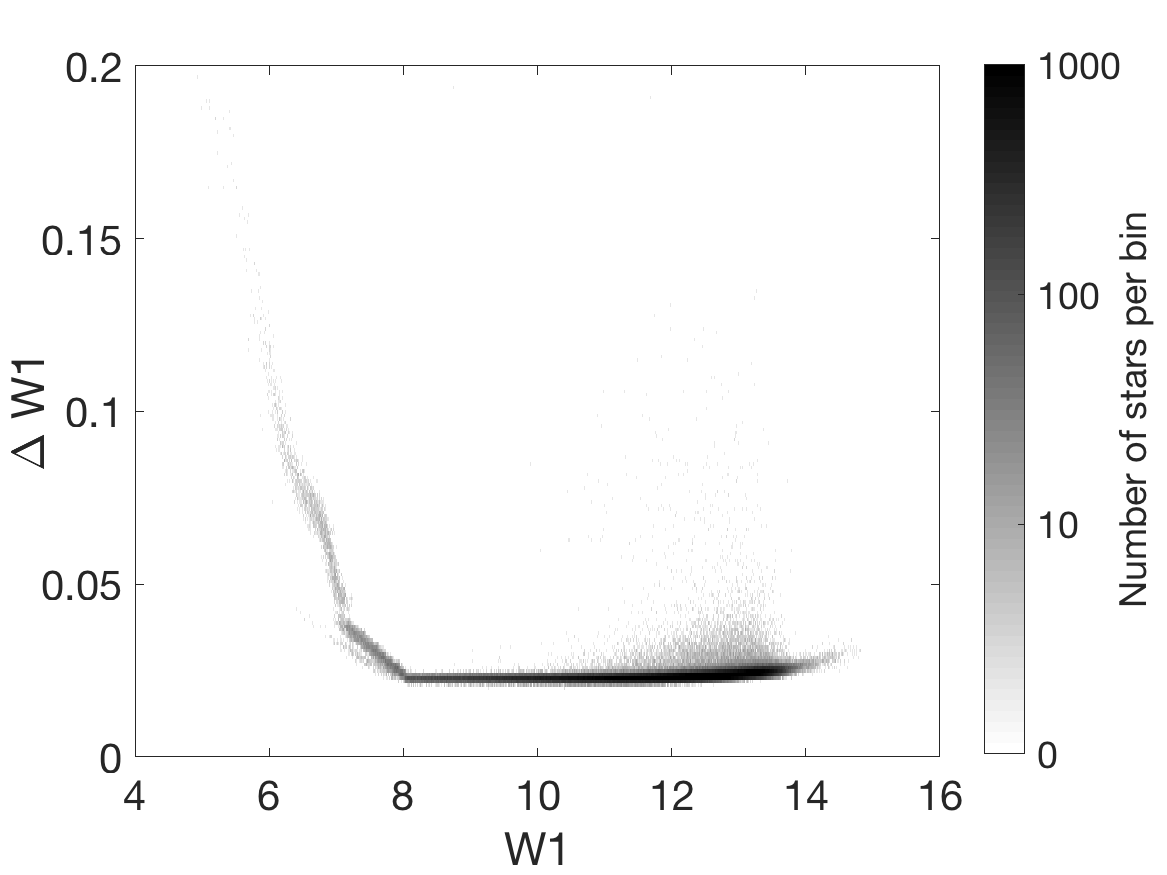
\includegraphics[width=0.8\textwidth]{deltaW1.pdf}
    \caption{Density plot of the number of stars per bin of the WISE photometric uncertainty as a function of the WISE magnitude W1.}
    \label{figDelta}
\end{figure}

The result of this photometric scattering applied to the data of Figure\,\ref{figScatterB} is shown in Figure\,\ref{figScatterC} -- the result is to significantly ``over scatter'' the simulated data compared to the observational data of Figure\,\ref{figScatterA}. All the features in W1--W2 in the scattered simulated data are too broad, as is the width of the M-dwarf branch in the J--W1 direction. The photometric confusion found in the observational data was more complex than just a simple normalised Gaussian distribution. It is expected that the photometric confusion seen is a product of multiple effects. At the very least, there is two levels of confusion in Figure\,\ref{figScatterA}. One that represents the minimally scattered, high-density population in the centre of the distribution, and the wider distribution of scattered stars that comprise the majority of what is seen in a colour-colour diagram (including the M-dwarf branch). \\ 

\begin{figure}[!ht]
    \centering
    \subfloat[]{\label{figScatterC}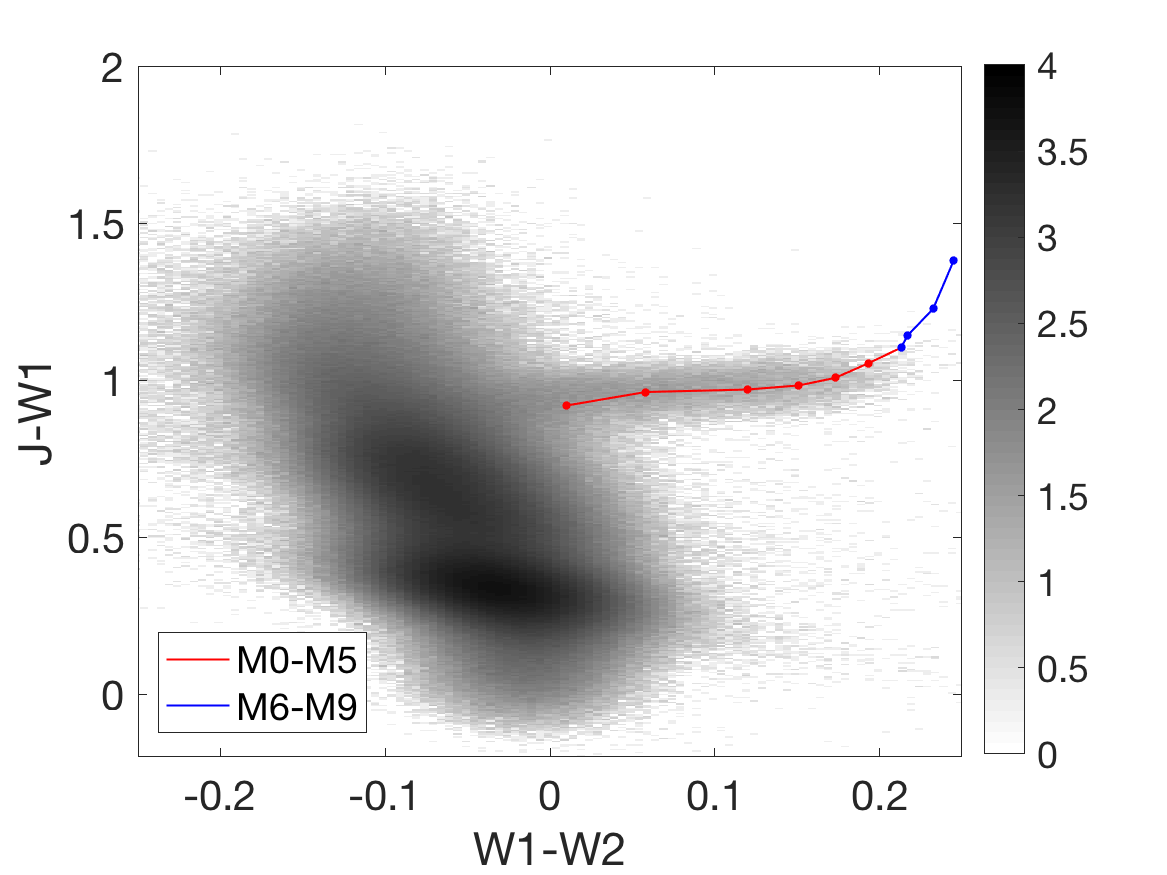
\includegraphics[width=0.8\textwidth]{Blur.png}}\\
    \subfloat[]{\label{figScatterD}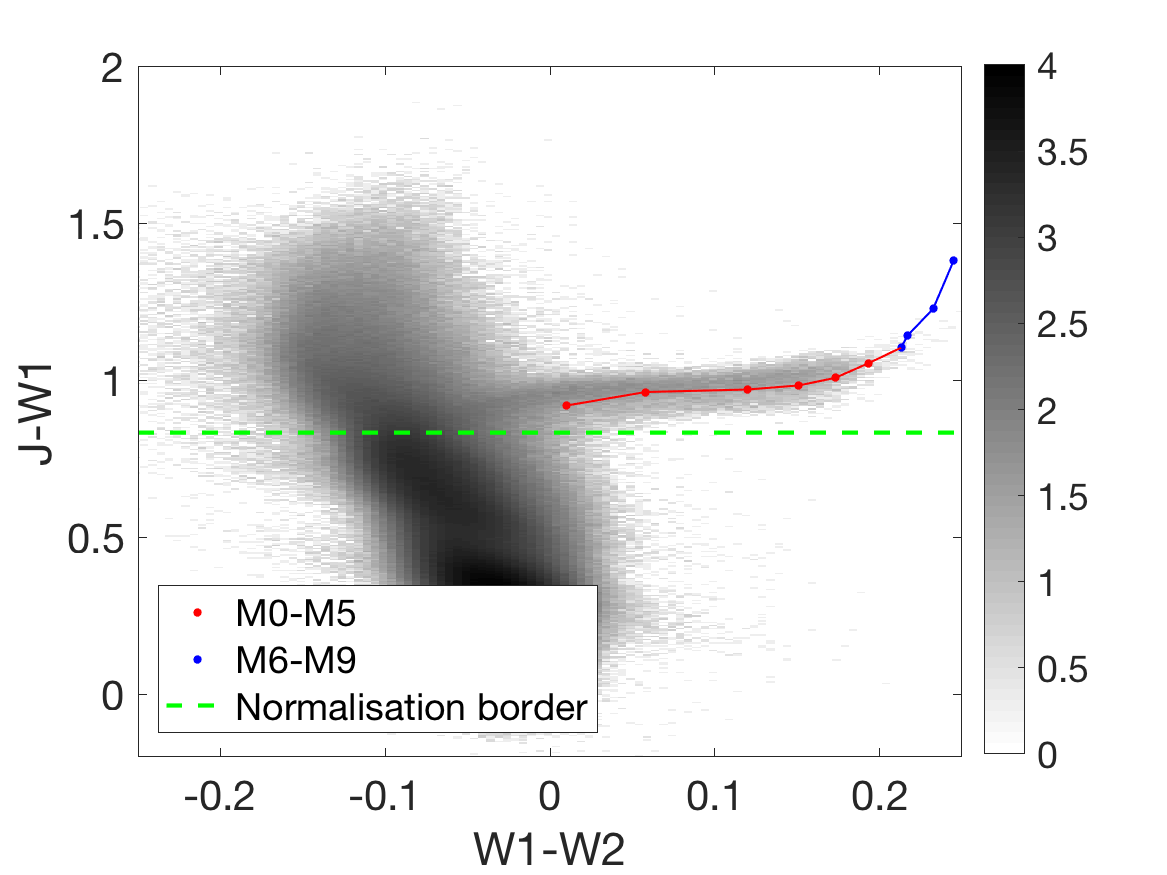
\includegraphics[width=0.8\textwidth]{galaxia.png}}
    \caption{Logarithmic source densities in the J--W1/W1--W2 plane for {\em Galaxia} data with two values of photometric scatter applied. Figure\,\ref{figScatterC} has the all the photometric scatter from the empirically determined relationships applied, while Figure\,\ref{figScatterD} has half of the scatter applied. Objects below the green horizontal line in Figure\,\ref{figScatterD} are used to normalise  {\em Galaxia} to observational data. The M-dwarf spectroscopic comparison sample from Section\,\ref{secSpecData} are overplotted in red and blue.} 
    \label{figPhotoScatter}
\end{figure}

As a response to this, two alternate methods were investigated. The first was to convolve the {\em Galaxia} colour data with a two dimensional kernel. This kernel was comprised of two, two dimensional Gaussians, which was hoped to simulate both populations mentioned above. This method has an added advantage over the previous method. The observational and synthetic datasets have different total populations. To accurately match the synthetic to the observational data, it needs to be scattered and normalised to match the observational. The level of scattering applied will also alter the amount that the synthetic population needs to be scaled by to match the observational data. This method determines both simultaneously as the kernel can scale the data it is convolved with. After empirically determining the lower and upper boundary conditions for each of the Gaussians comprising the kernel, a non-linear least-squares routine was applied to find the kernel that would produce a scattered synthetic population closest to the observation data by minimising the residuals between the two datasets. This resulted in a population significantly broadened, to the point that it no longer resembled the observational data at all. Visually determining the parameters needed for the kernel to scatter the {\em Galaxia} data produced data seen in Figure\,\ref{figKernel}.\\

\begin{figure}[!ht]
	\centering
    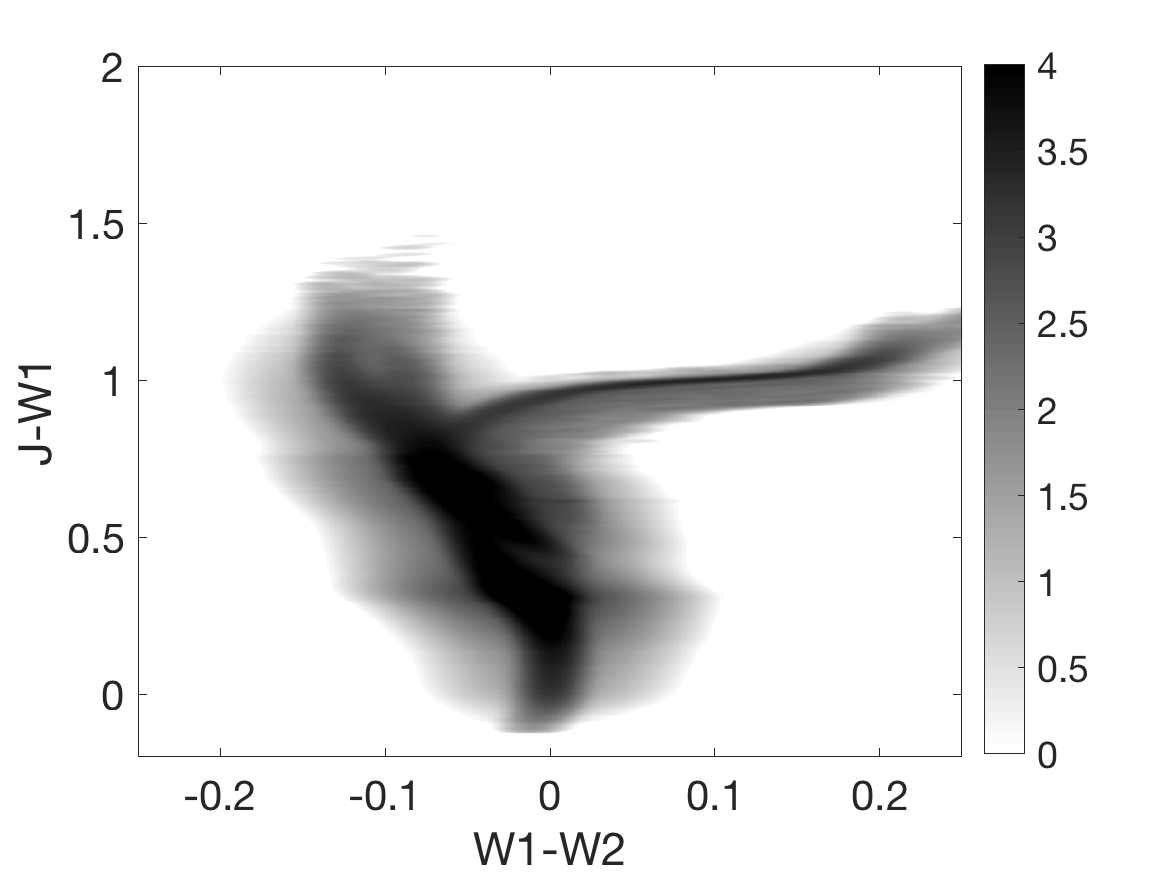
\includegraphics[width=0.8\textwidth]{Kernel.png}
    \caption{Density plot of the {\em Galaxia} dataset photometrically scattered by convolution with a 2-dimensional kernel.}
    \label{figKernel}
\end{figure}

The other method was to simply lower the fraction of the predicted photometric scatter applied to the simulated data. The amount required was empirically determined, so as to matched the observed distribution. It was found the initial scattering needed to be reduced by factors of near a half, and the resulting photometrically scattered data is shown in Figure\,\ref{figScatterD}.\\

Comparison of Figures\,\ref{figKernel} and \ref{figScatterD} show that while the kernel method does a better job of simulating the scale of both the populations mentioned above, it concentrates far too many stars in the high density regions, while the observational data shows a graduation between the two levels of scattering. The reduced photometric scatter method achieves a better simulated population in the regions that are most important - the high-density regions of hot stars and the M-dwarf branch, despite a lack of highly scattered stars at the ``edges''. Therefore the reduced photometric scatter method of Figure\,\ref{figScatterD} was used.
\subsection{Colour terms and offsets}
\label{secOff}
Comparison of the simulated and scattered data with the observational data, showed small -- but notable -- colour differences between {\em Galaxia} predicted colours and observed colours at the level of between several-hundredths to a few-tenths of a magnitude. This is not entirely surprising, inasmuch as the {\em Galaxia} predicted colours rely entirely on synthetic model atmospheres and model filter profiles. \\

``Benchmark'' features in the observed data were used to align the two sets of data. Figure\,\ref{figLandmark} shows example contours (rather than grey scales) of source density in J--W1/W1--W2 after these offsets were determined and applied. Offsets were determined using observed stars with G\,=\,9-14.5 from a number of features: the M-dwarf branch at J--W1$\approx$1; the G-dwarf clump at W1--W2\,$\approx$\,-0.03, J--W1\,$\approx$\,0.35; and the giant clump at W1--W2\,$\approx$\,-0.07, J--W1\,$\approx$\,0.7. As the aim of this work is to understand how selection criteria for M-dwarfs will be influenced by contamination, these offsets were weighted more heavily on the features nearest to the M-dwarf branch, as these are the source most likely to contaminate the M-dwarf selection. This is why in Figure\,\ref{figLandmark} the giant clump is better aligned than the G-dwarf clump. The offsets so determined and applied are reproduced in Table\,\ref{tabOffset}.\\

\begin{figure}
	\centering
    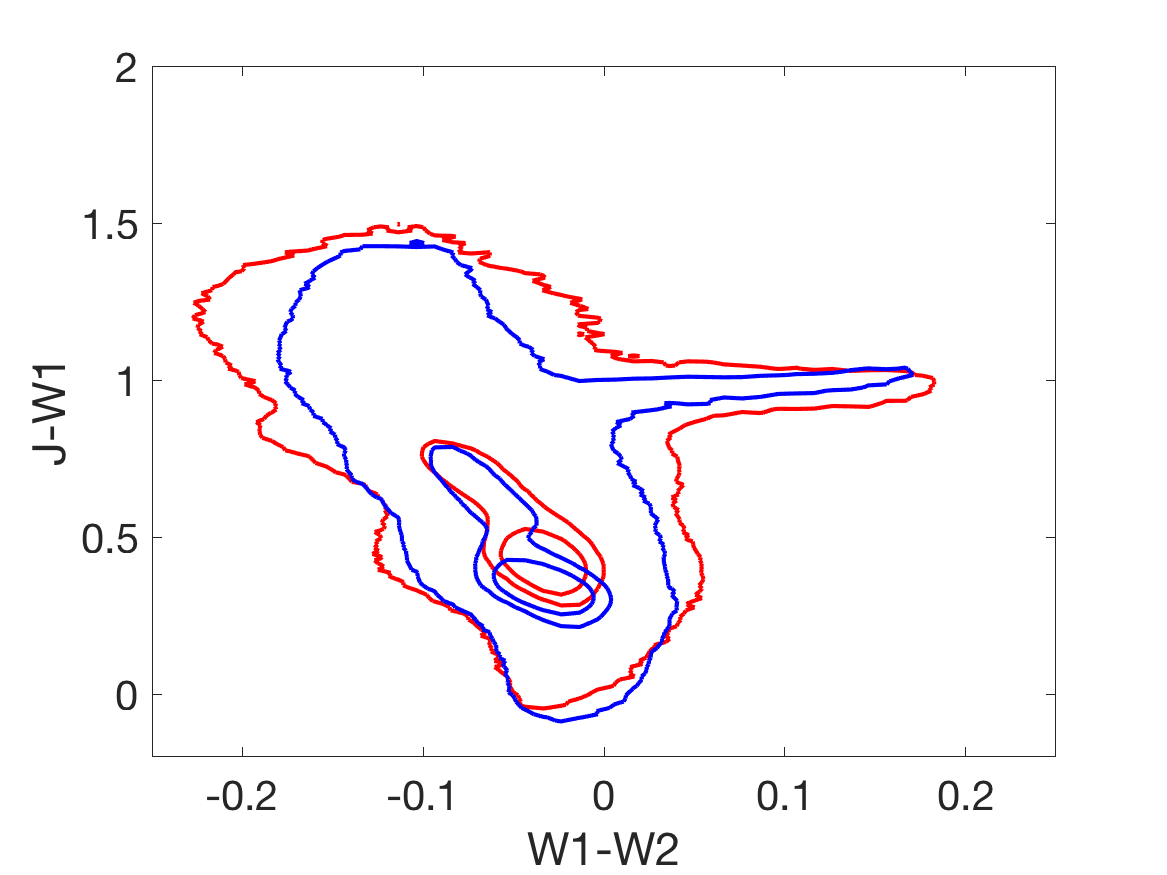
\includegraphics[width=0.8\textwidth]{Landmarks.pdf}
    \caption{Contours containing 30\%, 60\% and 99\% of the observational (in red) and simulated (in blue) data in J--W1, W1--W2. Offsets from Table\,\ref{tabOffset} have been used to align the simulation M-dwarf branch to its observational counterpart.}
    \label{figLandmark}
\end{figure}

\begin{table}
	\begin{center}
	\begin{tabular}{c c c c c} 
 		\hline
 		 G--J & G--H & G--K & G--W1 & G--W2\\
 		-0.01 & -0.02 & -0.05  & -0.05  & -0.1\\
        \hline
            & J--H & J--K & J--W1 & J--W2\\
            & -0.01 & -0.01 & -0.03 & -0.07\\
            \cline{2-5}
            \cline{2-5}
            &    & H--K & H--W1 & H--W2\\
            &    & 0 & -0.02 & -0.05\\
            \cline{3-5}
            \cline{3-5}
            &    &    & K--W1 & K--W2\\
            &    &    & -0.04 & -0.02\\
            \cline{4-5}
            \cline{4-5}
            &    &    &     & W1--W2\\
            &    &    &     & -0.025\\
 		\cline{5-5}
	\end{tabular}
    \caption{Zero-point colour offsets to align {\em Galaxia} colours with observed colours (in the sense that these offsets are added to synthetic colours).}
    \label{tabOffset}
	\end{center}
\end{table}

\subsection{Normalising {\em Galaxia} to the sky}
\label{secNorm}
Each {\em Galaxia} simulation run produces an arbitrary number of stars, (for this work, 4,931,764 were generated). To compare this synthetic {\em Galaxia} population with the observational {\em Gaia}/WISE/2MASS data, a normalisation between the two data sets was required. As noted above, while the colour offsets adopted (Table\,\ref{tabOffset}) aligned the M-dwarf branch, and features near that branch, in both datasets, there remain  a number of differences.\\

As noted above the G-dwarf clump does not align in Figure\,\ref{figLandmark}, even after the M-dwarf and giant clumps are aligned. This is believed to be due to limits on the reliability of the synthetic photometry adopted by {\em Galaxia}. Even after aligning for colour offsets there clearly remain higher-order colour terms.\\

Another difference between the observed and simulated data is seen in the M-giant region at J--W1$>$1 (see Figure\,\ref{figScatterA} and \ref{figScatterD}). The real galaxy produces a plume of objects with a wide distribution of colours, while {\em Galaxia} simulates a much narrower range. This is likely to be due to the significant variability and mass-loss present in this class of stars, resulting in intrinsic reddening and scattering in colour that is highly variable from source to source. In this region the simulated data also contains fewer stars than the observational data.\\

Given these differences it was felt that normalising {\em Galaxia} to the Galaxy using the total number of objects in both samples would not be the best way to proceed. Instead a normalisation determined from a comparison of the types of stars best represented in both datasets was used. {\em Galaxia} has been heavily tuned to match the observed Galaxy for relatively unreddened G-K dwarfs and giants. Therefore normalisation of the two samples was performed using the total number of stars 0.1\,mag below the M-dwarf branch in each colour-colour space (shown by the green horizontal lines in Figures\,\ref{figScatterA} and \ref{figScatterD}), and adopted a normalisation factor of 1.3918 to scale up the synthetic population to match the observational data. This means that, while the overall population will be close in number, specific regions may have differing numbers of stars.

\subsection{Connected component analysis}
\label{secCCA}
To identify the distribution of M-dwarfs and other key populations in both absolute magnitude and colour space, Connected Component Analysis (CCA; \citealt{1988Samet}) was used. CCA is a technique that identifies the pixels of a 2-dimensional image that comprise each component of the image. For this work, the images of interest are density images created by binning {\em Galaxia} simulated objects in colour-colour planes. Using this technique, groups of components that comprise the majority of the sample can be selected, excluding highly scattered components that comprise a small fraction of the total population but would inflate the selected region, adding significant numbers of stars not intended to be selected (i.e. non-M-dwarfs). For example, Figure\,\ref{figCCA} shows an example use of this technique for a density image of the adopted {\em Galaxia} M-dwarfs in the G--K/K--W2 colour-colour plane. The green contour is a rough measure of the region bound by all the {\em Galaxia} M-dwarfs while the red contour uses CCA to select 99.5\% of the M-dwarfs but excludes a number of the most photometrically scattered M-dwarfs. Losing 0.5\% of the M-dwarfs in the sample is an acceptable sacrifice to reduce the selected region and avoid as many non-M-dwarfs as possible.\\

Using the expected properties of M-dwarfs from \citet{2005Reid} (summarised in Table\,\ref{TabMK}) to identify {\em Galaxia} sources as M- or K-giants, or K-dwarfs (as well as the previously discussed criterion for M-dwarfs). CCA was used to identify regions that contain \textgreater\,97\% of each of these classes of object in the {\em Galaxia} simulations (see Figure\,\ref{figCCP}).\\

\begin{figure}
	\centering
    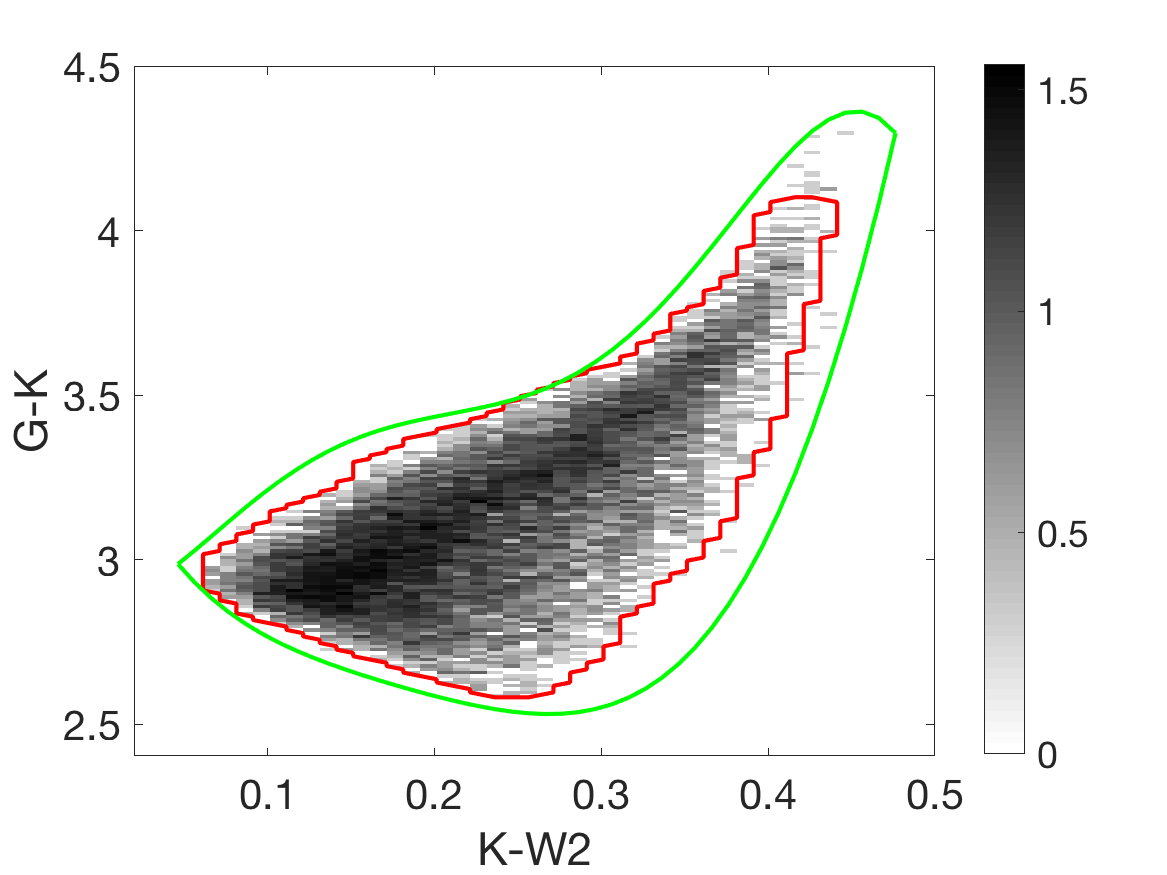
\includegraphics[width=0.8\textwidth]{CCA-2.pdf}
    \caption{Connected component analysis of the {\em Galaxia} M-dwarfs using the G--K and K--W2 colours. The red outline highlights the region defined as the largest component while the green line represents the boundary region around the entire {\em Galaxia} M-dwarf population for this colour plane.}
    \label{figCCA}
\end{figure}

\subsection{Completeness and contamination in simulations}
The simulated data allowed both the completeness and contamination (i.e. the false-positive rate) for each M-dwarf candidate selection method used, to be quantified. Simulated completeness is defined as the number of M-dwarfs selected, divided by the total number of M-dwarfs present in the simulation, and simulated contamination as the number of non-M-dwarfs identified by each set of criteria, divided by the total number of M-dwarfs and non-M-dwarfs selected by each set of criteria.
\section{Absolute Magnitude Selection}
\subsection{Selection criteria}
\label{secAbs}
Due to {\em Gaia} DR2's extensive catalogue of luminosities and distances, a primary selection of M-dwarfs via absolute magnitude is quite viable. Therefore, both the simulated data and spectroscopic comparison sample were used to examine the impact of a complete set of all-sky distance measurements.\\

A M$_G$/G--J colour-magnitude diagram was constructed using the simulated data (Figure\,\ref{figColMagA}), and the characteristics from Table\,\ref{TabMK}, plus CCA techniques, were used to identify and select the M and K dwarf, and M and K giant populations in this plane. It is clear that the risk of contamination of an M-dwarf sample by M and K giants is greatly diminished in absolute magnitude space, and the only significant issue in such a plane is the degree of K dwarf contamination as a function of an adopted upper luminosity limit in M$_G$ for M-dwarfs.\\

\begin{figure}
	\centering
    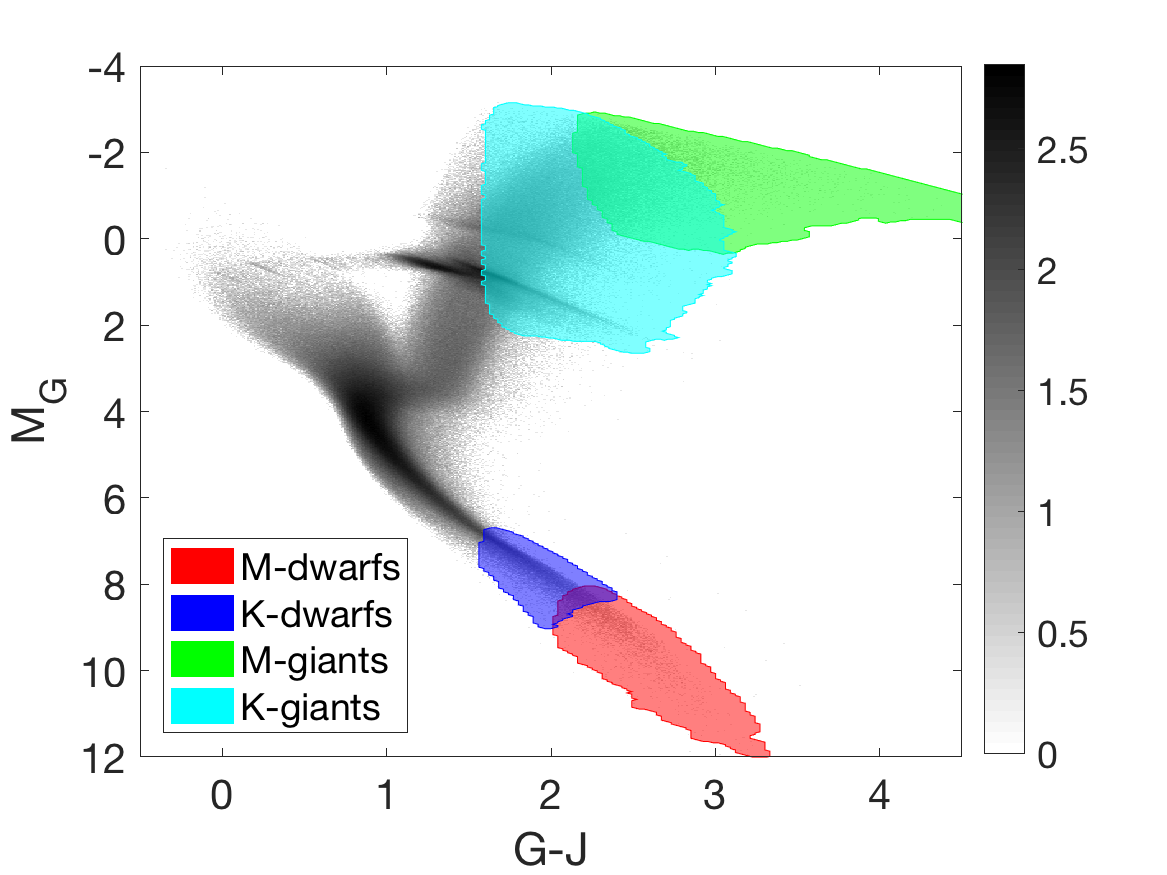
\includegraphics[width=0.8\textwidth]{AbsMag-G.png}
    \caption{Simulated M$_G$/G--J colour magnitude diagram for G\,\textless\,14.5. The K and M, dwarf and giant regions are identified using the criteria of Table\,\ref{TabMK}, and the overplotted CCA regions (complete to \textgreater\,97\%), where red is the simulated M-dwarfs, blue is the K-dwarfs, K-giants are in cyan, and M-giants are presented in green.}
    \label{figColMagA}
\end{figure}

Informed by these CCA regions, two M$_G$ cut-offs were chosen for M dwarf selection. An absolute magnitude limit of M$_G$\,\textgreater\,8.04, set at the bright end of the M-dwarf distribution, prioritising M-dwarf completeness, and a second limit which attempted to minimise K-dwarf contamination by setting the limit at M$_G$\,\textgreater\,8.86, the dim end of the K-dwarf distribution.\\

\begin{figure}
	\centering
	\captionsetup{width=.5\textwidth}
	\subfloat[A zoomed in image of the K to M dwarf boundary seen in Figure\,\ref{figColMagA}.]{\label{figColMagB}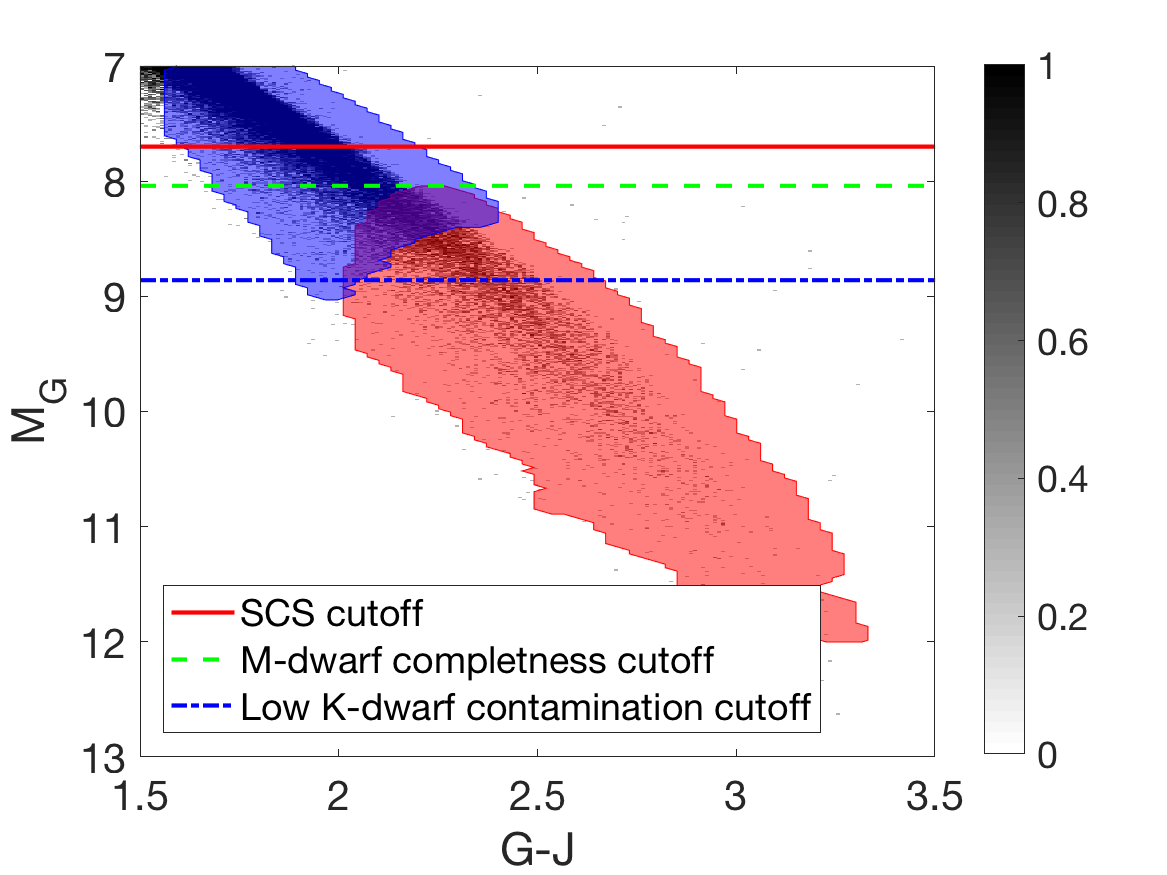
\includegraphics[width=0.6\textwidth]{MagCut_Close.png}}
	\subfloat[M$_G$/G--J colour magnitude diagram for the spectroscopic comparison sample.]{\label{figColMagC}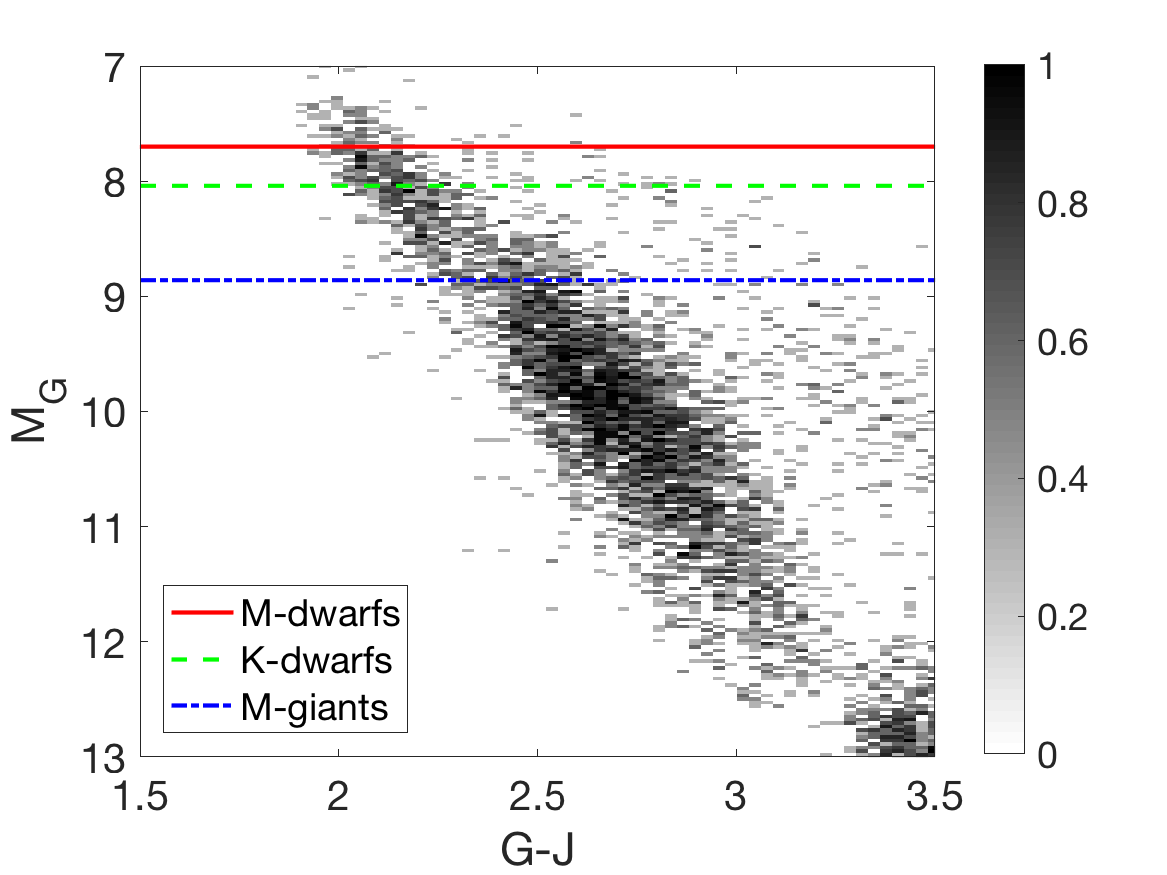
\includegraphics[width=0.6\textwidth]{WestAbsMag.png}}
    \caption{}
    \label{figColMag}
\end{figure}

A similar test was conducted using the spectroscopic comparison sample, cross matched with {\em Gaia} to obtain G-band photometry and parallaxes (and therefore absolute magnitude). An absolute magnitude limit of M$_G$\,\textgreater\,7.70 is required to select 97\% of the comparison sample (shown by the red solid line in Figures\,\ref{figColMagB} and \ref{figColMagC}). Neither the external completeness, nor levels of contamination, can be determined for this sample, since the selection function of the spectroscopic comparison sample itself is not well determined, and it doesn't contain non-M-dwarfs to examine contamination.\\

All three of these absolute magnitude limits are presented in Figures\,\ref{figColMagB} and \ref{figColMagC} as the red (M$_G$\,\textgreater\,7.70), green (M$_G$\,\textgreater\,8.04), and blue (M$_G$\,\textgreater\,8.86) horizontal lines.\\

Absolute magnitudes for the simulated data were derived from the distances generated for each star in the simulated population. Distances for the observational data (and hence absolute magnitudes), were derived from the inverse of the parallax. For samples of the bright, nearby stars being considered (M$_G$\,\textgreater\,7.70, G\,\textless\,14.5 implies M-dwarfs will lie at a maximum distance of 229\,$\pm$\,2pc), the typical uncertainties in Gaia DR2 data mean that the biases arising from obtaining a distance from an inverted parallax are completely negligible. While it is known that Gaia DR2 contains a number of stars with parallaxes that are either negative, and/or un-physically large, the number of such objects at these bright magnitudes is very small\footnote{See \citealt{2018Luri} for details on the Gaia DR2 parallaxes}.
\subsection{Completeness}
Investigation of these limits (see Table\,\ref{tabAbs}) found that the M$_G$\,\textgreater\,8.86 selection would achieve an unacceptably poor level of completeness (54.8\%), so it was not considered further. The M$_G$\,\textgreater\,8.04 selection significantly reduced the contamination rate of non-M-dwarfs by a factor of about 2. Moreover it does so while maintaining M-dwarf completeness at 99.96\%.\\

\begin{table*}
\hspace{-5mm}
	\begin{tabular}{ | c | c c c c | c c |} 
		\hline
        & \multicolumn{4}{c|}{Simulations} & \multicolumn{2}{c|}{Observations}\\
		M$_G$ & Meet & Total & Completeness & Contamination & Meet & Total\\
        limit & Criteria & M-dwarfs & (\%) & (\%) & Criteria & M-dwarfs\\
		\hline
        \textgreater\,7.70 & - & - & - & - & 76392 & -\\
        \textgreater\,8.04 & 39435 & 27583 & 99.96 & 29.4 & 55230 & 38992\\
        \textgreater\,8.86 & 18347 & 15259 & 54.8 & 16.8 & 24853 & 11234\\
		\hline
	\end{tabular}
    \caption{Absolute magnitude M-dwarf selections determined from West et. al (M$_G$\,\textgreater\,7.7) and {\em Galaxia} (M$_G$\,\textgreater\,8.04 \& M$_G$\,\textgreater\,8.86).}
    \label{tabAbs}
\end{table*}
Applying the M$_G$\,\textgreater\,7.70 and M$_G$\,\textgreater\,8.04 limits to the observational absolute magnitudes selects 76,392 and 55,230 stars respectively. For the {\em Galaxia} derived M$_G$\,\textgreater\,8.04 limit, a significantly greater number of stars are selected from the observational data than the 39,435 stars predicted from the simulated data. It is believed to be due to the localised discrepancies between the simulated and observational data, mentioned in Section\,\ref{secNorm}.\\

M-dwarf selection via absolute magnitude requires a bright limit somewhere in the range 7.70\,-\,8.04. Adopting the more luminous of these limits (derived from the empirical spectroscopic comparison sample) results in a more complete sample of M-dwarfs, without selecting an unfeasibly large number of stars to observe with FunnelWeb (\textless\,100,000). Applying this conservative luminosity selected criterion (hereafter `AbsCrit') selects 76,392 stars. This absolute magnitude limit applied to {\em Galaxia} selects all of the stars determined to be M-dwarfs. From this, and the spectroscopic derived limit, the M-dwarf completeness of the AbsCrit criterion is estimated to be 96.98-100\%.
\section{Colour selection}
As a complimentary selection criteria, it was decided to use the long-standing tradition in giant-dwarf discrimination of selecting colour-colour diagrams which aim to break degeneracies between stellar effective temperature and surface gravity. Specifically, colours sensitive to effective temperature were found for the horizontal axes, and those sensitive to surface gravity for the vertical axes. Of course, no such diagram is perfect and contamination will occur where different classes of star overlap. Most notably for this case, the low-temperature boundary of the M-dwarf regime which adjoins the (much more numerous) high temperature boundary of the late K-dwarf regime, as well as the less numerous lower boundary of the K- and M-giants. Even small amounts of photometric scatter, cosmic scatter and source confusion in these more numerous populations will lead to significant contamination of any M-dwarf selection.
\subsection{Stellar distributions}
After examining the many colour-colour combinations available from the six passbands used in this work, three were selected for use in this analysis. They are presented in Figure\,\ref{figCCP}. Each possesses distinct advantages.\\

\begin{itemize}
\item{{\em G--K/K--W2}: This plane displays the smallest levels of K-dwarf/M-dwarf overlap in all the colour-colour planes. In all colour-colour planes, K-dwarfs are the most significant source of contamination in the M-dwarf region, so selecting a colour-colour space that minimises this overlap greatly lowers the overall level of contamination.}
\item{{\em J--K/G--J}:  This plane has the advantage of using the G-band in the temperature-dependent horizontal axis to distribute the M-dwarf branch across a large colour range.}
\item{{\em J--K/W1--W2}: This has the advantage of using a colour on the horizontal axis for which both bands come from the same survey, telescope and instrument, which reduces issues associated with cross-matching, and systematics between surveys with different sensitivities, instrument resolution and data processing.}
\end{itemize}

\begin{figure}
	\centering
	\vspace{-3cm}
    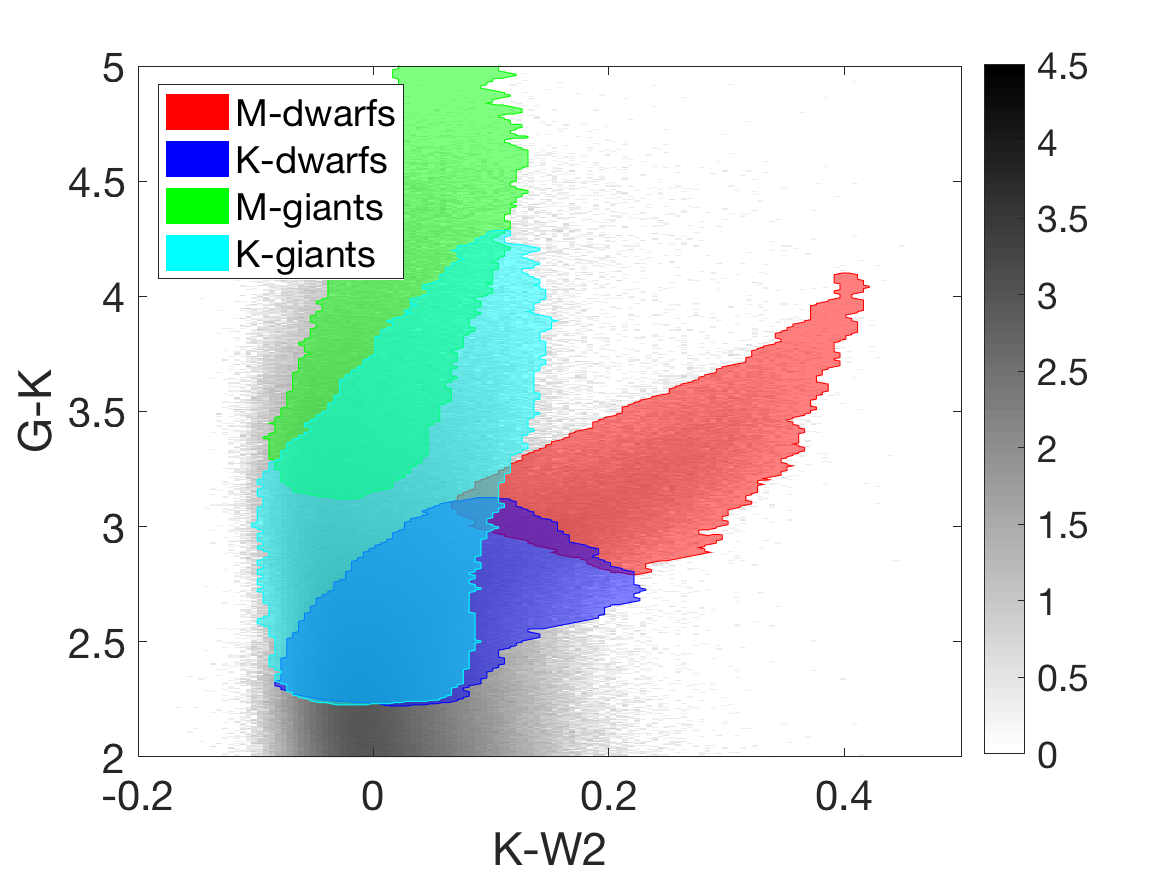
\includegraphics[height=0.35\textheight]{GKKW2.png}\\
    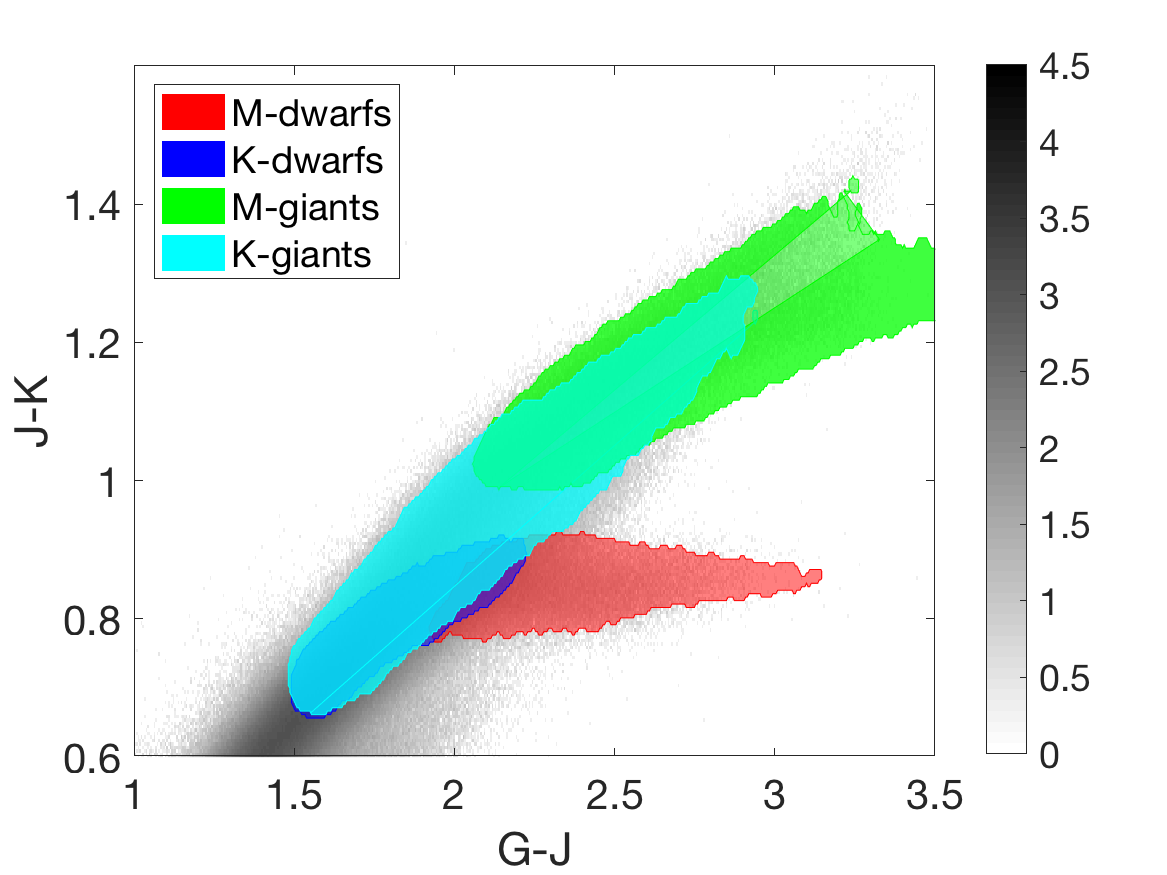
\includegraphics[height=0.35\textheight]{JKGJ.png}\\
    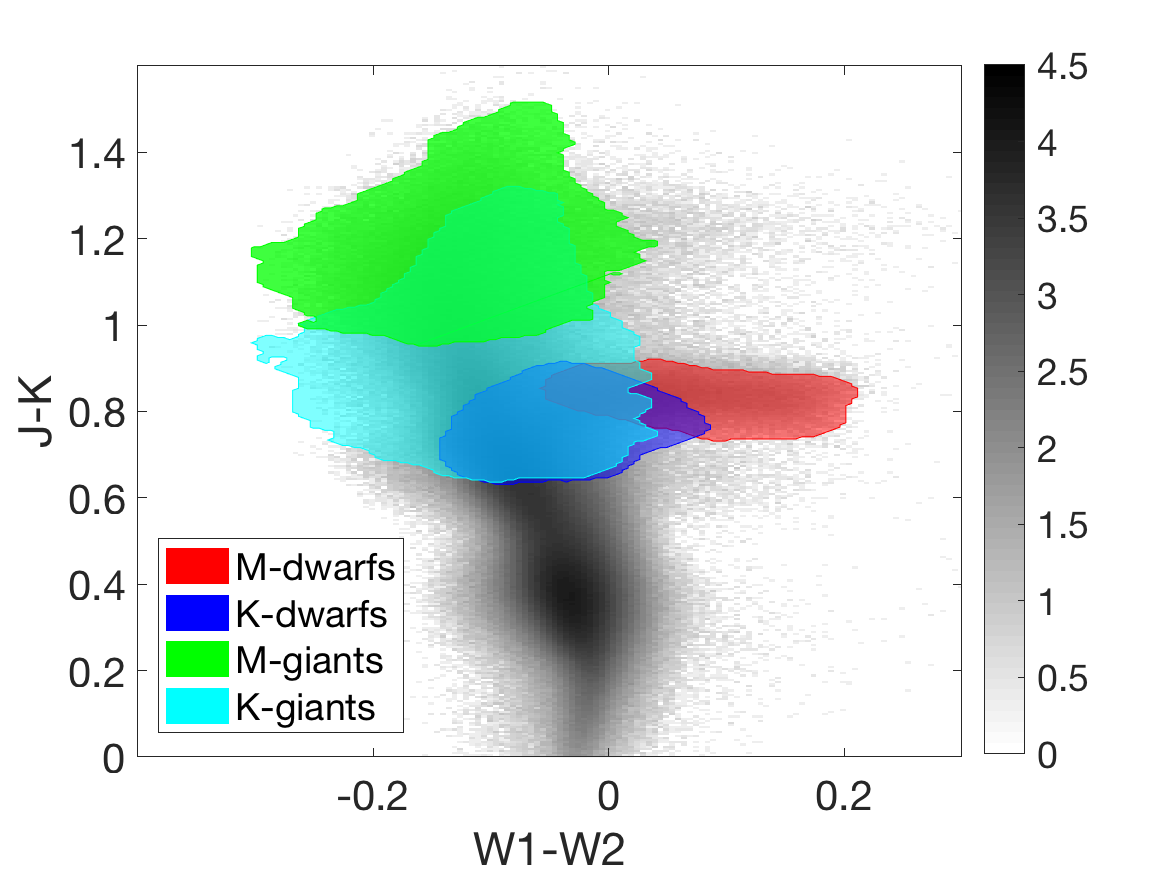
\includegraphics[height=0.35\textheight]{JKW1W2.png}\\
    \caption{The three colour-colour spaces chosen for this work. Coloured regions highlighting the four classes of stars of importance to this work, as identified by the CCA analysis described in Section\,\ref{secCCA}. In each case these connected regions contain \textgreater\,97\% of the relevant class in the {\em Galaxia} simulation. Red - M-dwarfs; Blue - K-dwarfs; Cyan - K-giants; Green - M-giants.}
    \label{figCCP}
\end{figure}
\subsection{Selection criteria}
Guided by the principle of keeping the photometric selection criteria as simple as possible. The initial work used simple rectangular selection regions in colour-colour space, bounded by the maxima and minima of the CCA regions for M-dwarfs. However, these were quickly found to be unsatisfactory -- there was simply too much contamination at the boundaries between between classes of object, which do not follow either vertical or horizontal lines in these planes.\\

\begin{figure}
	\centering
    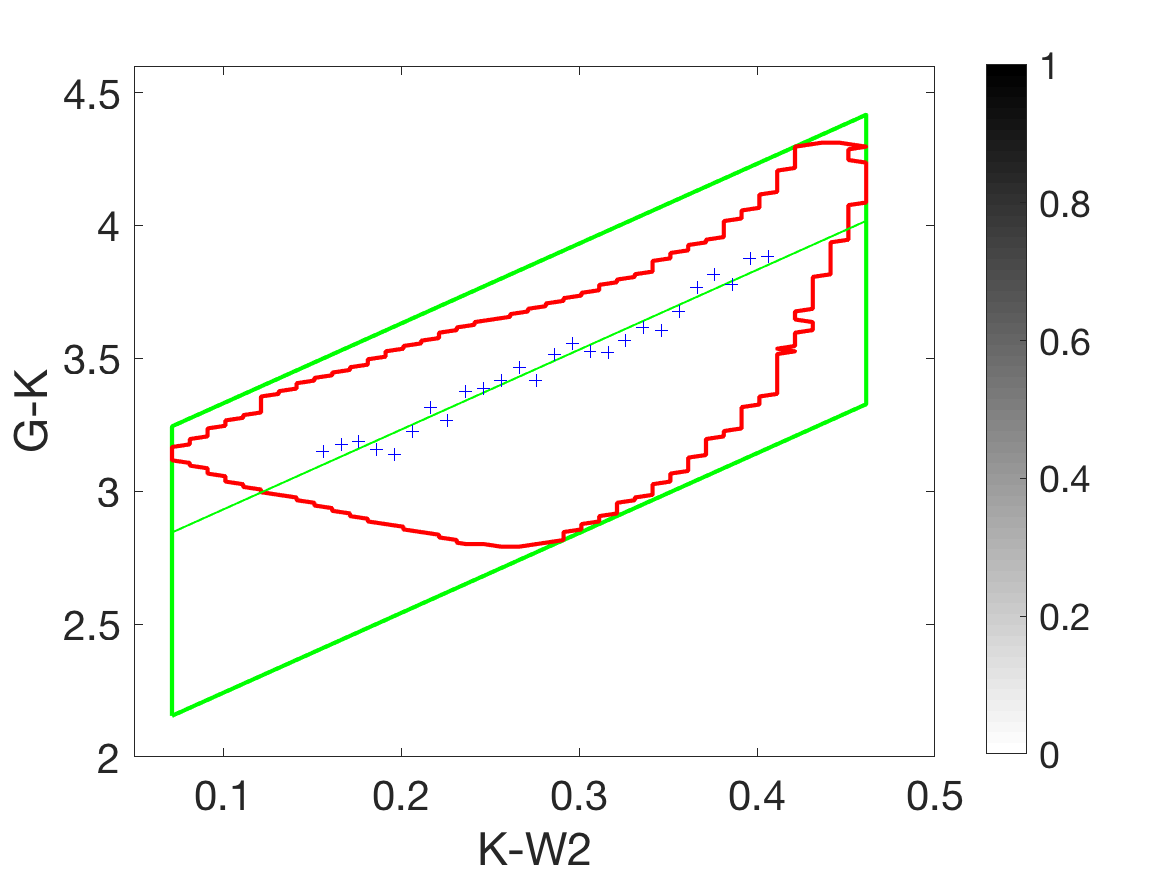
\includegraphics[width=1\textwidth]{Parallelogram.pdf}
    \caption{Construction of a parallelogram selection region using the CCA information seen in Figure\,\ref{figCCA}. The red line bounds the primary connected component, the blue crosses represent the G-K values of highest density for the middle 60\% of the K-W2 bins. The thin green line is a linear fit through the blue crosses and the thick green lines represent the parallelogram formed from the intersection of the polynomial with the minimum and maximum K--W2 values from the primary connected component.}
    \label{figPara}
\end{figure}

The next simplest model (i.e. parallelograms) were utilised as the simplest polygon able to represent the M-dwarf region. The data in the M-dwarf CCA region was binned along each horizontal axis and fitted a linear polynomial to the middle 60\% of points in each bin. Figure\,\ref{figPara} shows an example of this for the data plotted in Figure\,\ref{figCCA}.\\

\begin{table}[]
    \centering
    \begin{tabular}{|r|}
        \hline
        High completeness criteria\\
        \hline
        K-W2\,\textgreater\,0.061\\
        K-W2\,\textless\,0.441\\
        G-K\,\textgreater\,3.26(K-W2)\,+\,2.124\\
        G-K\,\textless\,3.26(K-W2)\,+\,3.209
        G-J\,\textgreater\,2.011\\
        G-J\,\textless\,3.441\\
        J-K\,\textgreater\,-0.010(G-J)\,+\,0.723\\
        J-K\,\textless\,-0.010(G-J)\,+\,0.927
	    W1-W2\,\textgreater\,-0.059\\
        W1-W2\,\textless\,0.221\\
        J-K\,\textgreater\,-0.051(W1-W2)\,+\,0.720\\
        J-K\,\textless -0.051(W1-W2)\,+\,0.938\\
        \hline
    \end{tabular}
    \caption{Colour selection comprising the `high completeness' criteria.}
    \label{eqHC}
\end{table}

This results in the three groups of ``high completeness'' criteria shown in Table \ref{eqHC}, which are shown in Figure\,\ref{figBox} overplotted on the observational data as by the red parallelograms. Looking at the numbers selected by each criterion (Table\,\ref{TabColSelect}) two conclusions can be reached.\\

\begin{table*}
\begin{center}
	\begin{tabular}{| c | c | c | c || c | c | c || c |}
		\hline
        Data & A & B & C & A \& B & A \& C & B \& C & A \& B \& C\\
        \hline
        Simulated & 109310 & 193384 & 129136 & 66186 & 73507 & 67248 & 58264 \\
        Observational & 245736 & 329228 & 223686 & 108238 & 124243 & 121205 & 94145 \\
        \hline
\end{tabular}
\caption{Comparison of the number of stars selected from each colour criterion comprising Table\ref{eqHC}. `A' represents the G--K/K--W2 criterion; `B' is the J--K/G--J criterion and `C' is the J--K/W1-W2 criterion.}
\label{TabColSelect}
\end{center}
\end{table*}
Firstly, the J--K/G--J colour plane (B) selects significantly more stars than the other two colour regions. However, the combination of this colour criterion with either of the other two criteria (A \& B or B \& C) selects fewer stars than the combination without it (A \& C). The combination of all three reduces the number of selected stars even further, to just 60\% of the smallest colour selection (A). As stated previously, photometric confusion limits the ability to use a single colour range to define a single class of star. However, a contaminant in one colour is not necessarily going to be present as a contaminant in other colours. Selecting M-dwarfs via multiple colours and requiring a candidate star to fall within all of the M-dwarf colour ranges will reduce the number of contaminants selected. At the same time, selection by too many colour ranges might throw out a non-trivial number of M-dwarfs, lowering M-dwarf completeness. It was decided that three colour-colour planes would be a reasonable balance.\\

It was then made a requirement that an object must satisfy all three of these colour-colour criteria to be considered a candidate M-dwarf. Secondly, the total number of stars within the simulated colour regions are much less than the corresponding regions in the observational data. Of particular note is the B \& C combination, in which the simulated numbers are, at worst, 9\% smaller than the other combinations, while the observational population is roughly 50\% greater than the other populations. This was expected (see Section\,\ref{secNorm}), however this highlights the extent to which specific regions might differ between the simulated and observational datasets.\\

\begin{figure}
	\centering
	\vspace{-3cm}
    \subfloat[]{\label{figBoxA}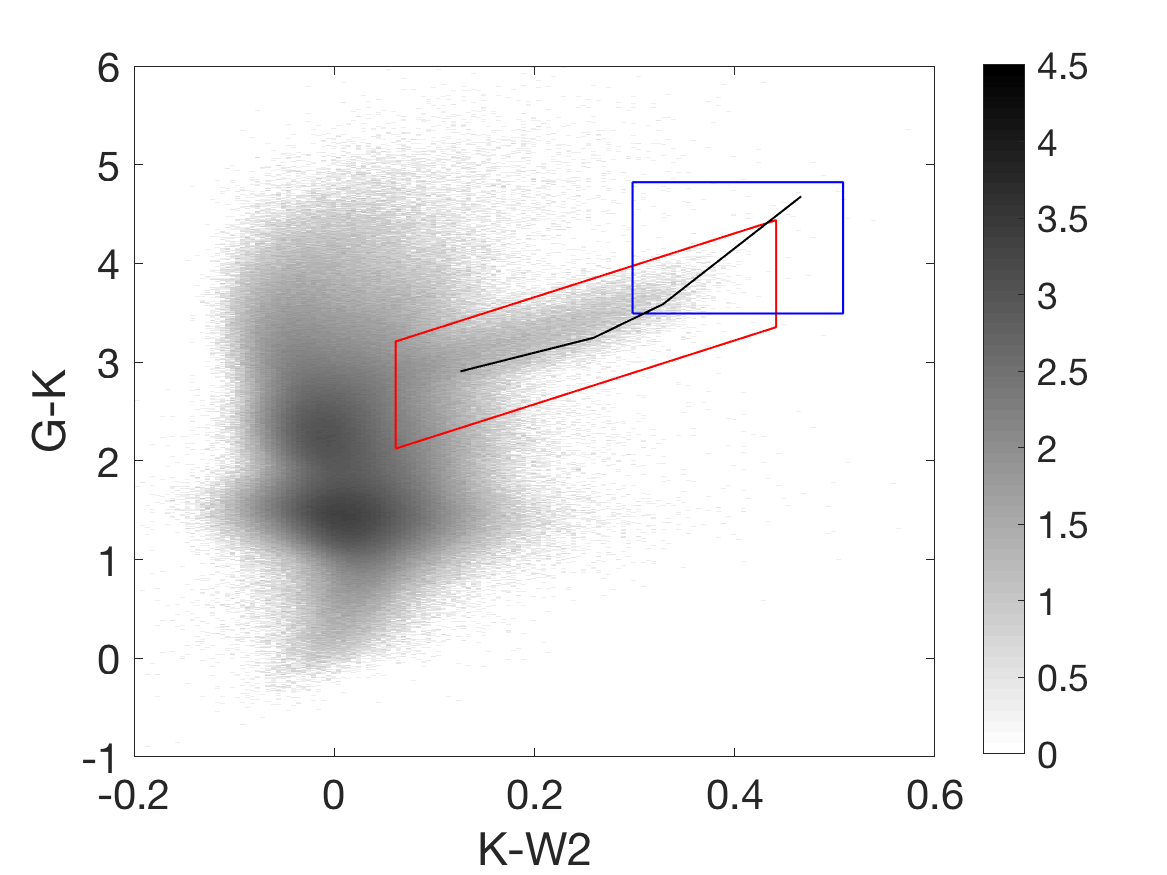
\includegraphics[height=0.3\textheight]{resultsGKKW2.png}}\\
    \subfloat[]{\label{figBoxB}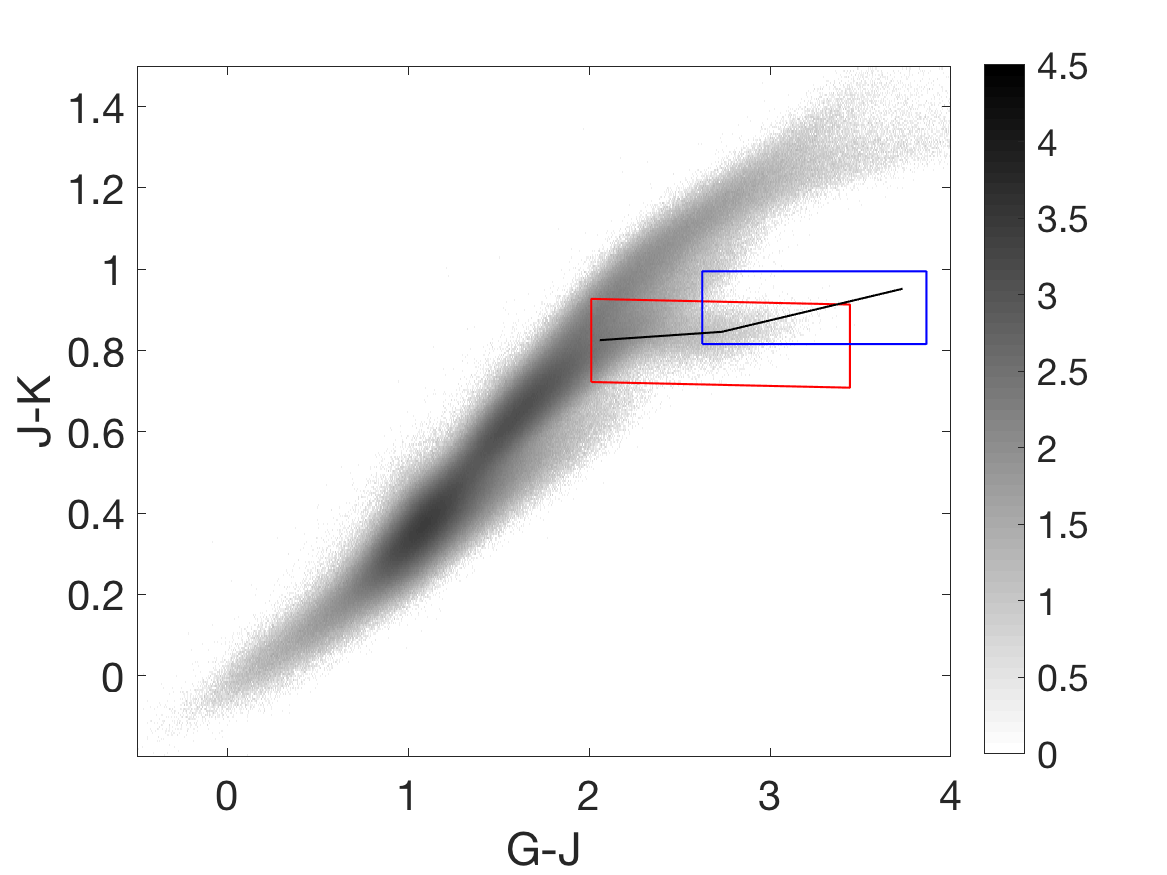
\includegraphics[height=0.3\textheight]{resultsGJJK.png}} \\
    \subfloat[]{\label{figBoxC}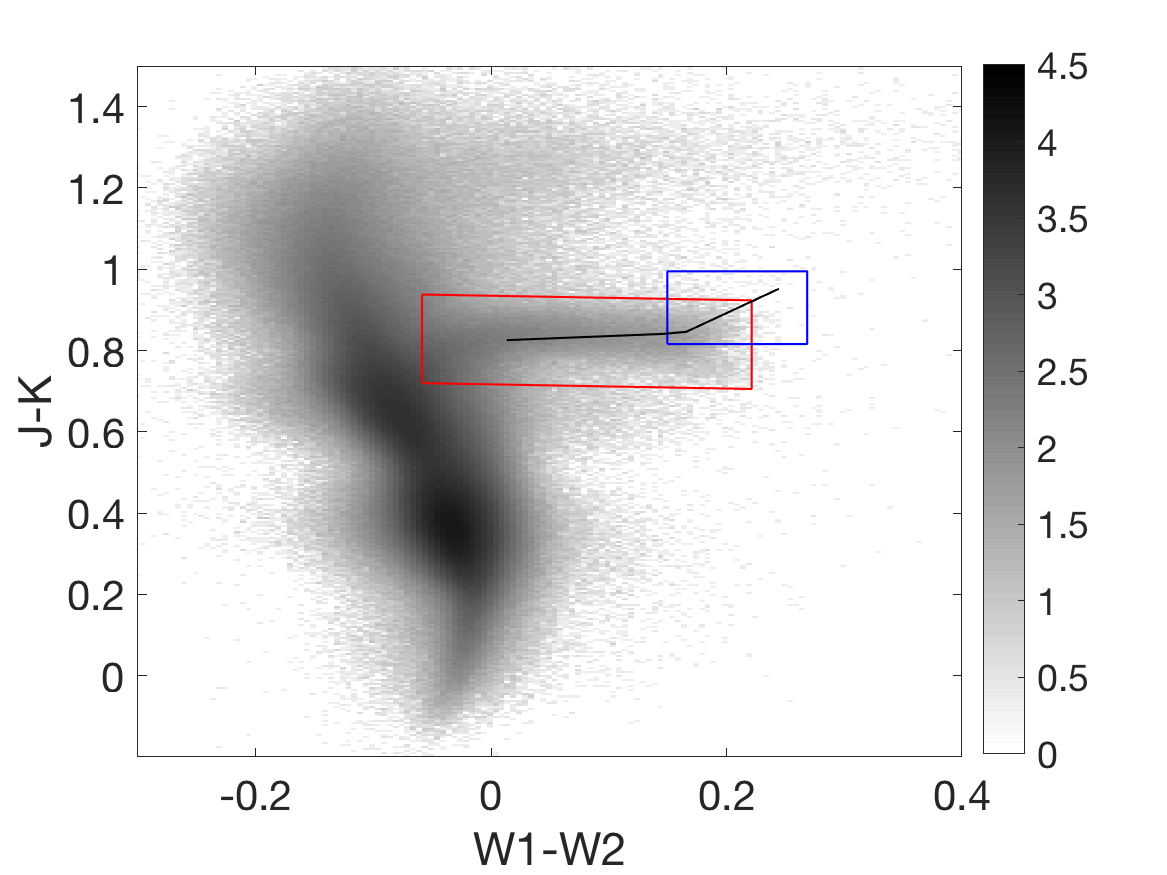
\includegraphics[height=0.3\textheight]{resultsW1W2JK.png}}
    \caption{Colour-colour density plots of {\em Gaia}/WISE/2MASS photometry with the colour regions selected by the ColCrit criteria for G\,\textless\,14.5 in red. The blue box contains the M6-M9 stars that are absent from the selected colour regions. The black line represents the M-dwarf median colour values from Table\,\ref{TabLookup}.}
	\label{figBox}
\end{figure}
While the completeness of this combined set of criteria is very high (99.3\%), the number of simulated non-M-dwarfs significantly outnumbers the number of simulated M-dwarfs, with most of the non-M-dwarf contamination arising at the transition point from K-dwarfs/giants to M-dwarfs.\\

The conditions that define these sets of criteria consist of four colour limits per colour-colour plane. The most influential is the blue limit of the colour used as the measure of temperature on the x-axis of each colour-colour plane, which is the transition point between K-stars and M-dwarfs. This limit will affect both the contamination levels, and what fraction of the total number of M-dwarfs (in particular, M0) are within the selected region. Moving this limit to bluer values will increase the number of M-dwarfs selected, but will add a substantial amount of K-stars, more than the number of M-dwarfs added. Reducing the size of the selected region by moving this limit to redder values will reduce the K-star contamination, at the expense of the M-dwarf completeness. The other three limits, while important, are not as crucial as the blue x-axis limit.\\

To reduce this contamination rate a second set of ``low contamination'' criteria were constructed, by moving the lower x-axis boundary conditions of each colour region to reduce the number of stars selected. The stars excluded from the colour region will include both M-dwarfs and non-M-dwarfs. The optimal colour region will exclude as many non-M-dwarfs as possible while minimising the amount of M-dwarfs that are lost. The range spanned across the x-axis by each of the selection criteria was divided into twenty bins and the lower boundary condition was moved in by one bin at a time and determine the number of M-dwarfs and non-M-dwarfs in the selected region. This was calculated for all three colour spaces and all permutations. An ``optimal'' set of colour ranges can then be chosen by maximising $f$ in Equation\,\ref{eqFrac}, where $M_{tot}$ is the total number of stars identified in {\em Galaxia} as M-dwarfs, $M_{sel}$ is the number of {\em Galaxia} identified M-dwarfs within the selected colour region and $S_{sel}$ is the total number of stars within the selected colour region.\\

\begin{equation}
\hspace{3cm}f = \frac{M_{sel}}{M_{tot}} \times \frac{M_{sel}}{S_{sel}}
\label{eqFrac}
\end{equation}

The criteria that results are given in Table\,\ref{eqLC}. These result in non-M-dwarfs comprising $\approx$38\% of the total selected sample, while maintaining M-dwarf completeness at 95\%.\\


\begin{table}[]
    \centering
    \begin{tabular}{|r|}
        \hline
        Low contamination criteria\\
        \hline
        K-W2\,\textgreater\,0.099\\
        K-W2\,\textless\,0.441\\
        G-K\,\textgreater\,3.26(K-W2)\,+\,2.247\\
        G-K\,\textless\,3.26(K-W2)\,+\,3.232
        G-J\,\textgreater\,2.154\\
        G-J\,\textless\,3.441\\
        J-K\,\textgreater\,-0.010(G-J)\,+\,0.721\\
        J-K\,\textless\,-0.010(G-J)\,+\,0.926
	    W1-W2\,\textgreater\,-0.017\\
        W1-W2\,\textless\,0.221\\
        J-K\,\textgreater\,-0.051(W1-W2)\,+\,0.718\\
        J-K\,\textless\,-0.051(W1-W2)\,+\,0.936\\
        \hline
    \end{tabular}
    \caption{Colour selection comprising the `low contamination' criteria.}
    \label{eqLC}
\end{table}

Late M-dwarfs (i.e. later than M5 -- shown in blue in Figure\,\ref{figSubtypes}) appear off the red end of the {\em Galaxia} M-dwarf branch, because {\em Galaxia} cannot simulate them (Section\,\ref{secModel}). This can be seen from Figure\,\ref{figBox} in which the observed M-dwarf photometric sequences are shown as the black curves. To select these late M-dwarfs would necessitate moving the ``vertical'' red cut-off in K--W2, G--J and W1--W2 in Table\,\ref{eqHC} to a redder value, as well as also allowing slightly redder colours in G--K and J--K. \\

This number of such very late M-dwarfs is expected to be small. Nonetheless, a supplementary set of selection criteria to cover the full M-dwarf range, was developed using the median colours and r.m.s. scatter for M6-M9 spectroscopic comparison data (Section\,\ref{secSpecData}). As this area is far from the main sources of contamination (K-stars and giants) using a rectangle to bound this region is adequate, and these late M-dwarf colour regions are indicated by the blue boxes in Figure\,\ref{figBox}.\\

\begin{table}[]
    \centering
    \begin{tabular}{|r|}
        \hline
        Late M-dwarf criteria\\
        \hline
        K-W2\,\textgreater\,0.298\\
        K-W2\,\textless\,0.508\\
        G-K\,\textgreater\,3.493\\
        G-K\,\textless\,4.823\\
        G-J\,\textgreater\,2.625\\
        G-J\,\textless\,3.864\\
        J-K\,\textgreater\,0.816\\
        J-K\,\textless\,0.995\\
	    W1-W2\,\textgreater\,0.150\\
        W1-W2\,\textless\,0.268\\
        \hline
    \end{tabular}
    \caption{Colour selection comprising the `late M-dwarf' criteria.}
    \label{eqLM}
\end{table}

Therefore, selecting the full range of M-dwarfs requires both sets of criteria. As such the definition of the colour criteria (``ColCrit'') is the combination of criteria in Tables\,\ref{eqHC} and \ref{eqLM}. Adding these late M-dwarfs will only add 249 new stars, a trivial number compared to the main criteria. However, their addition is important for completeness. The results of this final colour criteria are reported in Tables \ref{tabCritA} and \ref{tabCritB}.\\

\begin{table}
	\begin{tabular}{ | c | c c c c | } 
		\hline
		& \multicolumn{4}{c|}{Simulations}\\
		\cline{2-5}
		Criteria & Meet & Total & Completeness & Contamination\\
		         & Criteria & M-dwarfs & (\%) & (\%)\\
		\hline
		High completeness & 58655 & 27757 & 99.6 & 52.7\\
		Low contamination & 37257 & 26483 & 95 & 28.9\\
		\hline
	\end{tabular}
    \caption{Simulated predictions for M-dwarf selection using the ``high completeness'' and ``low contamination'' criteria. ``Meet Criteria'' numbers are all objects in either sample that meet the criteria. The ``Total M-dwarf'' numbers are simulated objects identified as M-dwarfs that are selected by each set of criteria, and ``Completeness'' is the percentage of that number of the total number of simulated M-dwarfs. ``Contamination'' is the percentage of simulated objects that ``Meet Criteria'' but are not simulated M-dwarfs.}
    \label{tabCritA}
\end{table}
\begin{table}
    \centering
	\begin{tabular}{ | c | c c c | } 
		\hline
		& \multicolumn{3}{c|}{Observations}\\
		\cline{2-4}
		Criteria & Meet     & \multicolumn{2}{c|}{Predicted M-dwarfs}\\
		         & Criteria & (Number)  & (\%)\\
		\hline
		High completeness & 94479 & 27757\,-\,44710 & 29.4\,-\,47.3\\
		Low contamination & 53220 & 26483\,-\,37830 & 49.8\,-\,71.1\\
		\hline
	\end{tabular}
    \caption{Observational predictions for M-dwarf selection using the ``high completeness'' and ``low contamination'' criteria. ``Meet Criteria'' numbers are all objects in either sample that meet the criteria. ``Predicted M-dwarfs'' are the extreme ranges for numbers of objects in the Observational sample that ``Meet Criteria'' and could be real M-dwarfs (see text).}
    \label{tabCritB}
\end{table}
\subsection{Contamination in observations}
Applying both selection criteria to the observational sample selects the number of objects that ``Meet Criteria'' listed in Tables \ref{tabCritA} and \ref{tabCritB}. The first point that is apparent from these numbers is that the number of observed objects that meet the ColCrit criterion is around 60\% higher than the number predicted by the {\em Galaxia} simulation -- i.e. 94,479 vs 58,655.\\

As mentioned in Section\,\ref{secNorm}, it was found to be problematic to obtain a single normalisation between the {\em Galaxia} and observational data sets, with different regions of the simulated colour-colour plane requiring different normalisations. The chosen overall normalisation was one based on the population of main sequence stars with J--W1\,\textless\,0.67, where {\em Galaxia} has been most tuned to accurately match the observed Galaxy.\\

There are two ways to look at the difference between the total number of objects selected by each criteria in the simulated data and in observed data. At one extreme, the number of simulated M-dwarfs could be correct and the simulations fail to reproduce the way the real world scatters non-M-dwarfs into the colour selection criteria regions. At the other extreme the simulations could be correctly predicting the total number of objects in the colour selection regions, and under-predicting the total M-dwarf stellar population -- in this situation, the best estimate of the number of M-dwarfs to be identified will be the number of observed objects that meet the criteria, times one-minus-the-contamination-rate derived from the simulations. The fact that the difference between the predicted and observed number counts is significantly smaller for the ``low contamination'' sample (which digs into the K-dwarf, K-giant and M-giant regime much less than the ``high completeness'' sample) suggests the former is more likely. However the latter cannot be ruled out.\\

Therefore Table\,\ref{tabCritB} contains two estimates for the total number of M-dwarfs predicted to be found in the observed sample. They are the extreme bounds that arise from these two assumptions. Therefore the contamination rate range is 52.7-70.6\%.\\

Whether the level of contamination with a sample selected by either criteria is acceptable for M-dwarf selection will depend greatly on the total number of candidates identified and the resources available for follow-up of those candidates. If the total number identified is $\sim$100,000 objects and they can be observed spectroscopically as part of a survey targeting 1,000,000 stars a year (as is the goal of the {\em FunnelWeb} survey), then the cost of a contamination rate of 52.7\% is perfectly acceptable. If they are being followed-up by observation one-at-a-time, then that cost would be prohibitive.\\

The ``high completeness'' criteria selects 58,655 stars with 27,757 of these expected to be M-dwarfs, while the ``low contamination'' criteria selects 37,257 stars, and 26,483 are predicted to be M-dwarfs. While the ``low contamination'' criteria has a lower contamination, just like the three absolute magnitude limits determined in Section\,\ref{secAbs}, the total numbers of stars selected is sufficiently low that adopting the more complete criteria, despite it's contamination levels, was considered the best option.\\

Therefore the adopted colour based criteria (hereafter ``ColCrit'') is the combination of criteria from Tables\,\ref{eqHC} and \ref{eqLM}, and is designed to maximise the selection of M-dwarfs, at the cost of higher non-M-dwarf contamination. This criteria is predicted to select 99.6\% of all M-dwarfs, at the cost of 52.7\% of the objects selected not actually being M-dwarfs.
\section{Comparison of criteria}
\label{secCombined}
To determine the level of refinement that can be obtained by adding the ColCrit colour based criteria to the AbsCrit luminosity based criteria, it was decided to compare the samples of objects selected by each criteria. Looking at the ColCrit selected stars in absolute magnitude space (Figure\,\ref{figHiCompNew}), it can be seen that despite using multiple colour planes to reduce contamination (particularly giants), colour selection cannot avoid significant levels of contamination from distant, but bright, objects that have apparent magnitudes similar to M-dwarfs. These contaminants represent around 35\% of the stars selected by the ColCrit criterion (Table\,\ref{tabAbsNew}).\\
\begin{figure}
\centering
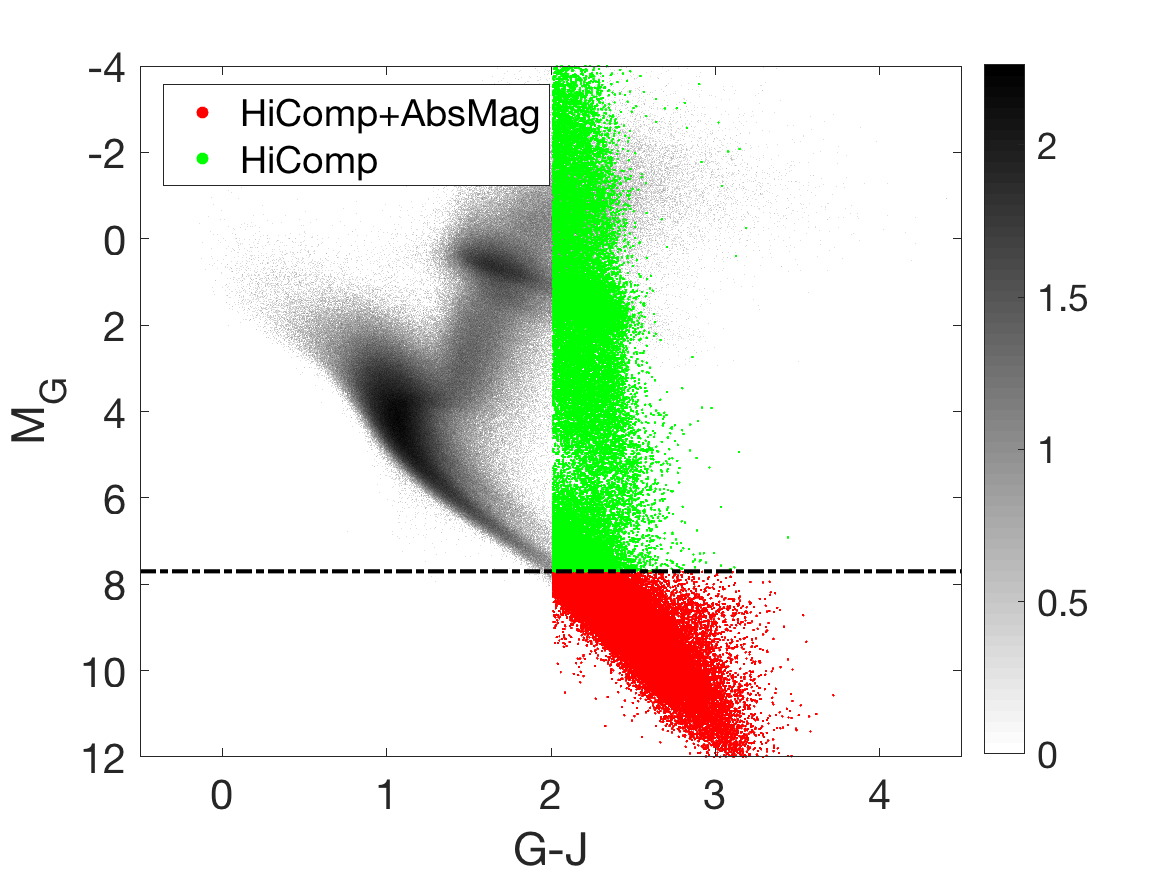
\includegraphics[width=1\textwidth]{AbsColour.png}
\caption{Selection of stars via the ColCrit criterion in M$_G$/G-J. The black dash-dotted line indicates the absolute magnitude limit of the AbsCrit criterion. ColCrit stars that agree with the AbsCrit criterion are in red and those that disagree are in green.}
\label{figHiCompNew}
\end{figure}

Conversely, the colour distribution of stars selected by the AbsCrit criterion (Figure\,\ref{figAbsNew}), shows that the majority of absolute magnitude selected stars fall within (or close to) the colour regions defined by ColCrit (the black dash-dotted line), indicating general agreement. 61,903 stars would be selected by both criteria, with the stars selected by AbsCrit, but not by ColCrit being a estimation of the minimum contamination for the AbsCrit criterion, which came out as 18.97\%. These excluded stars can be put into two categories - those in the K/M boundary region that are very close to the ColCrit colour boundaries which may in fact be M-dwarfs, and those that are in colour regions too far from the M-dwarf branch to realistically be photometrically scattered M-dwarfs.\\

\begin{figure}
\centering
\vspace{-3cm}
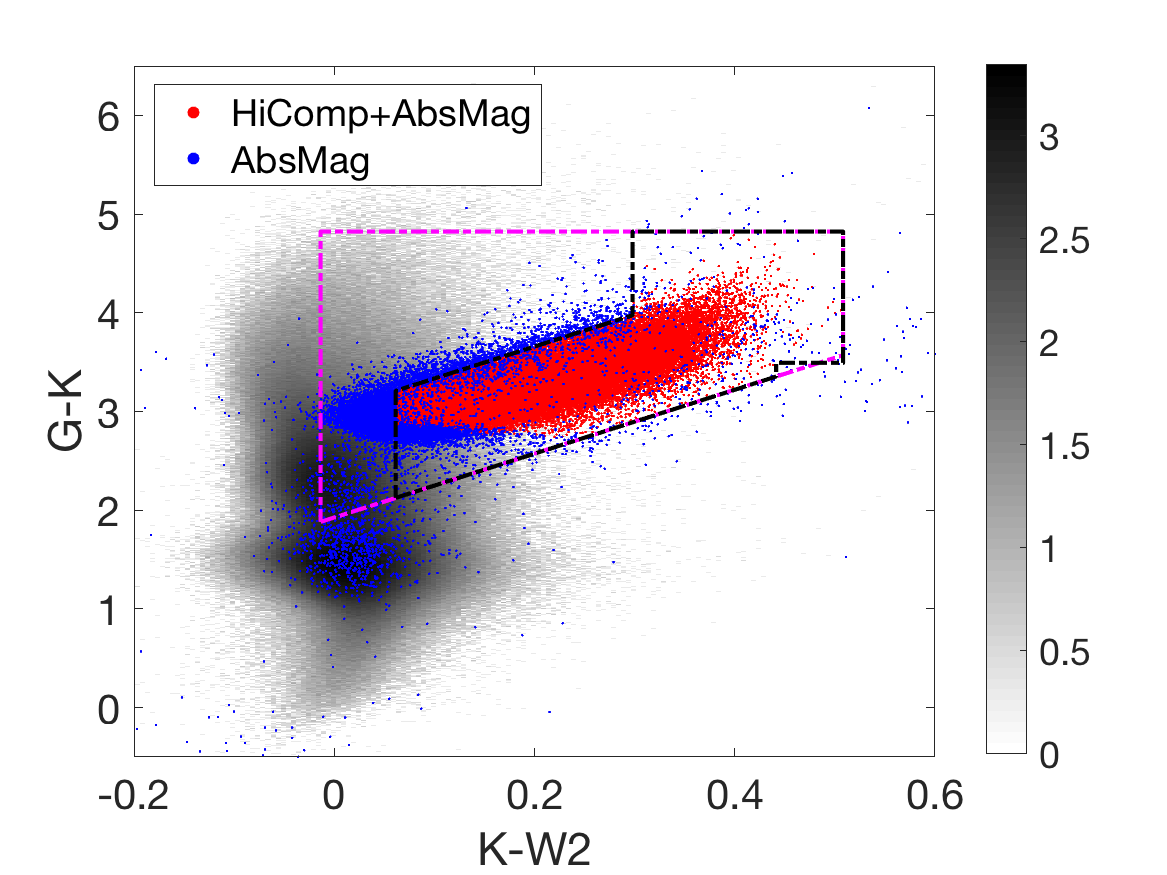
\includegraphics[height=0.3\textheight]{AbsGKKW2.png}\\
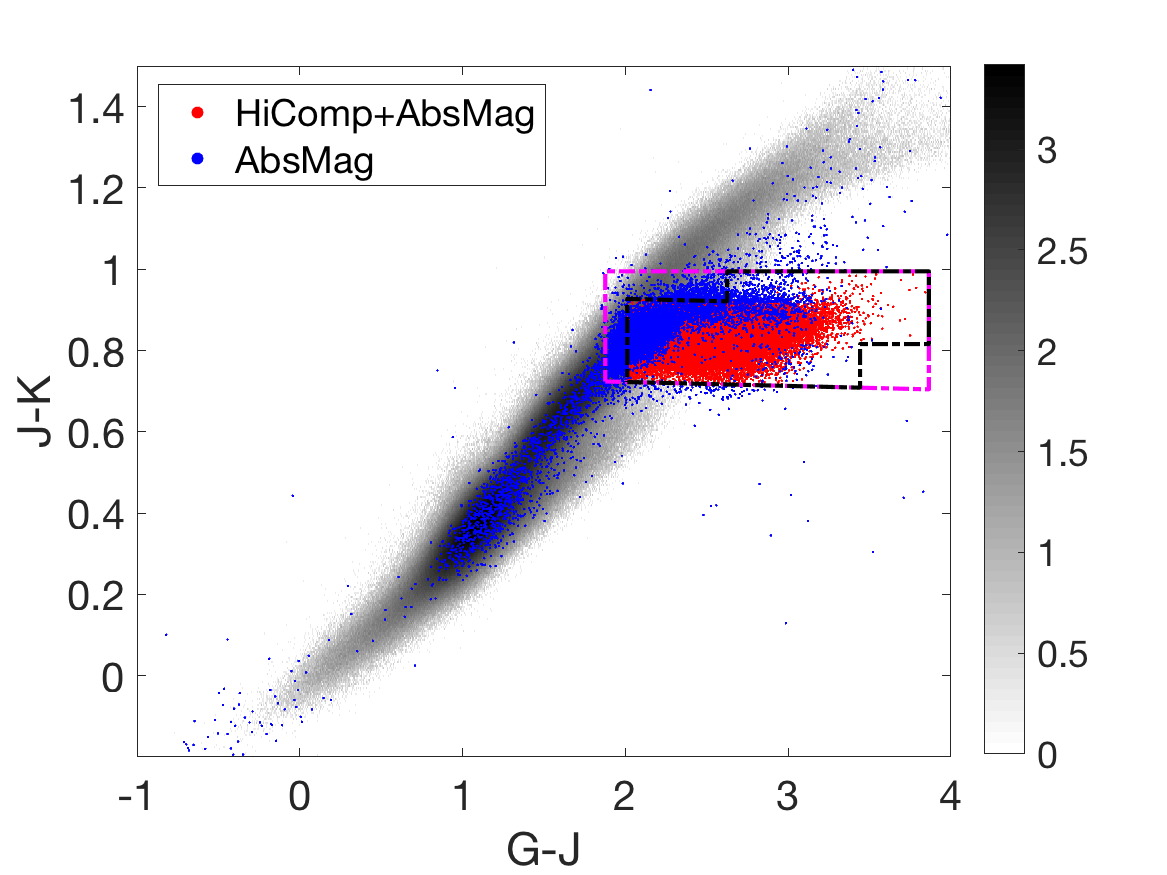
\includegraphics[height=0.3\textheight]{AbsJKGJ.png}\\
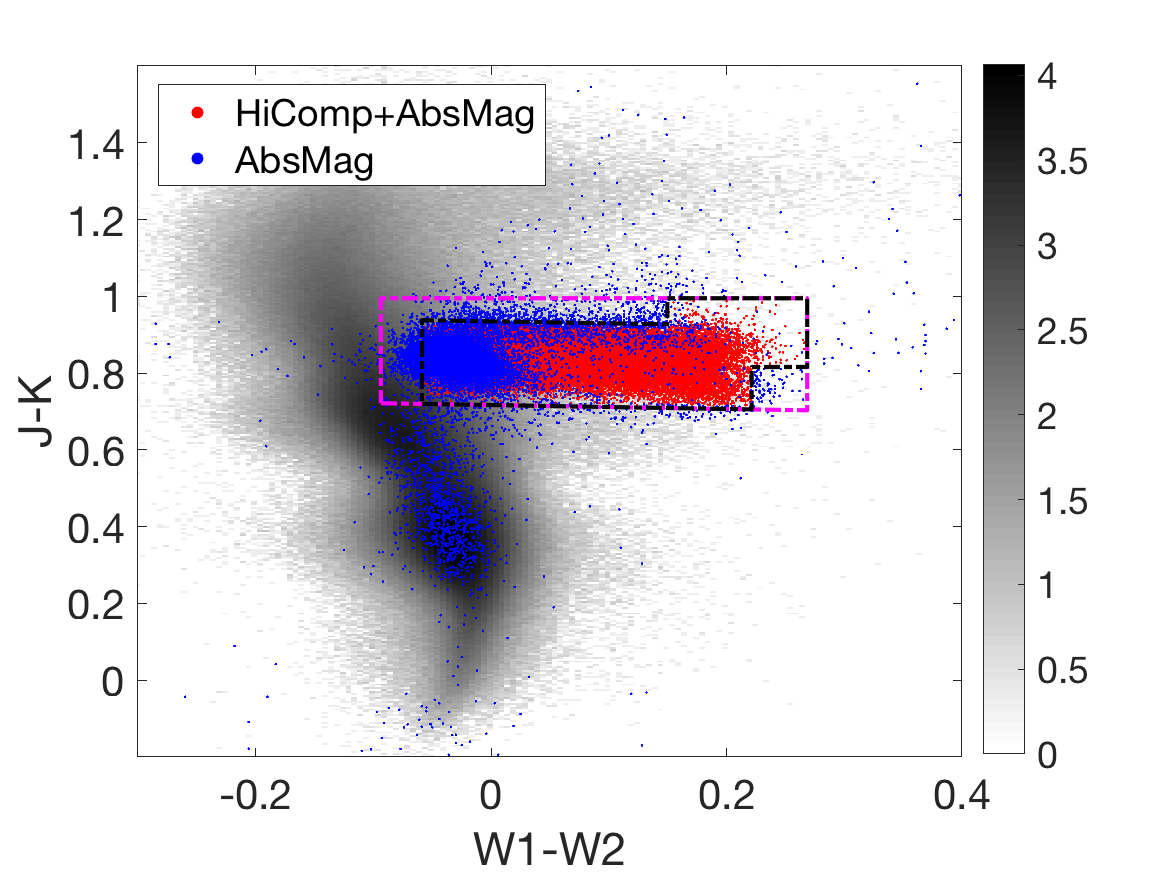
\includegraphics[height=0.3\textheight]{AbsJKW1W2.png}
\caption{The colour distribution of stars selected by the AbsCrit criterion. Stars selected by AbsCrit and ColCrit are in red and those selected by AbsCrit alone are in blue. The black dash-dotted outline highlights the colour region selected by the ColCrit criteria for the each colour plane and the magenta dash-dotted line represents the colour region of the criteria determined from both ColCrit and AbsCrit.}
\label{figAbsNew}
\end{figure}

\begin{table}
    \centering
	\begin{tabular}{ | c | c c c | }
		\hline
		Criteria & Total & Lower Limit & Completeness\\
		         & Selected & Contamination (\%) & (\%)\\
		\hline
		AbsCrit & 76392 & 18.97 & 96.98-100\\
		ColCrit & 94479 & 34.48 & 99.3\\
        Combined & 61903 & - & 99.0\\
		\hline
	\end{tabular}
    \caption{Comparison of the AbsCrit and ColCrit criteria. Stars selected by AbsCrit were analysed in colour space and the absolute magnitudes of stars selected by ColCrit were also investigated. ``Lower Limit Contamination'' refers to the percentage of the stars selected by one criteria that are not selected by the other criteria. Completeness is derived from the spectroscopic comparison sample for AbsCrit and the simulated data for ColCrit and CombinedCrit sample.}
    \label{tabAbsNew}
\end{table}
Table\,\ref{tabAbsNew} highlights that while both criteria are expected to select the majority of M-dwarfs (\textgreater99\%), both have significant levels of contamination, albeit of different types. As such, it is expected that the combination of colour and absolute magnitude selection will compensate for the weaknesses of each selection method and provide the best results.\\

The combination of absolute magnitude and colour as the final criteria allows for a less restrictive colour selection, increasing completeness while not substantially increasing contamination. In particular, expanding the colour limits closer to the giant region would select more giants, but it will be offset by the ability to separate giants from dwarfs in absolute magnitude. The final criteria (presented in Table\,\ref{eqFin}), which is called CombinedCrit, are trapezoids bounding the distribution of stars by both ColCrit and AbsCrit, plus the absolute magnitude limit of AbsCrit. The colour regions of this criteria can be seen as the magenta dash-dotted region in Figure\,\ref{figAbsNew}.\\ 

\begin{table}
    \centering
    \begin{tabular}{|r|}
        \hline
        CombinedCrit criteria\\
        \hline
    	M$_G$\,\textgreater\,7.7\\
        K-W2\,\textgreater\,-0.014\\
        K-W2\,\textless\,0.508\\
        G-K\,\textgreater\,3.236(K-W2)\,+\,1.882\\
        G-K\,\textless\,4.823
        G-J\,\textgreater\,1.876\\
        G-J\,\textless\,3.864\\
        J-K\,\textgreater\,-0.010(G-J)\,+\,0.724\\
        J-K\,\textless\,0.995
        W1-W2\,\textgreater\,-0.094\\
        W1-W2\,\textless\,0.268\\
        J-K\,\textgreater\,-0.051(W1-W2)\,+\,0.722\\
        \hline
    \end{tabular}
    \caption{Colour selection comprising the final M-dwarf selection criteria.}
    \label{eqFin}
\end{table}

This final set of criteria selects 74,091 stars. It excludes 1,139 outliers that were selected by AbsCrit, but have colours well outside the region expected for M-dwarfs. It also excludes 1,162 objects that are within some, but not all, of the colour regions. Investigation of the outliers shows that 140 have been spectroscopically observed (and mostly classified as white dwarfs) - the majority have no spectroscopic classification. There may be some genuine M-dwarfs within these unclassified objects, however their position in colour space and the requirement that no object have more than one 2MASS crossmatch within 3" of each {\em Gaia} object (which reduces the chance that the object is not a binary system of an M-star and a hotter star) makes this is unlikely.
\subsection{Absolute Magnitude Selection for objects unmatched between {\em Gaia}-2MASS-WISE}
\label{secExcl}
As mentioned in Section\,\ref{secObsData}, 638,845 objects in the initial sample of 8 million {\em Gaia} DR2 targets with G\,\textless\,14.5, were not able to be cross-matched between {\em Gaia}, 2MASS and WISE. This could be viewed as leading to a potential incompleteness of $\sim$8\% for the selection of M-dwarfs. While these unmatched objects (hereafter ``NoColCrit'') can not be classified via colour selection, their absolute magnitudes can be determined. Applying the M$_G$\,\textgreater\,7.70 limit to this sample, selects 11,679 potential M-dwarfs. The absence of colour information for these targets means that their selection as potential M-dwarfs can not be as confident as for those that pass the CombinedCrit criteria. However, their inclusion in a combined CombinedCrit+NoColCrit brings the total selection to just under 86,000 objects, which is still under the 100,000 objects deemed a reasonable target for {\em FunnelWeb}.

\section{Conclusion}
Investigations of the synthetic and observational photometric samples of M-dwarfs determined three absolute magnitude limits. Due to the relative number of stars that each set of criteria selects and the expected rate of observation of current and upcoming surveys, a focus on completeness is more beneficial than reducing the number of contaminants selected alongside the M-dwarfs. As such, an absolute magnitude limit of M$_G$\,\textgreater\,7.70 for the absolute magnitude based criteria (AbsCrit) as this is the brightest limit and therefore will select the most stars, maximising the M-dwarf completeness. Applying this criteria to the observational dataset selects a sample of 76,392 stars.\\

A completeness focused, colour based, criteria (ColCrit) selects 94,479 potential M-dwarfs. While the contamination levels in this criteria are not trivial (52.7\%), multi-object spectroscopic surveys, such as {\em FunnelWeb} will be able to observe all candidate stars in a relatively short period of time and spectroscopically confirm which are M-dwarfs and which are contaminants.\\

Comparison of the absolute magnitude based AbsCrit, and colour based ColCrit, selected samples, highlight that a selection solely by absolute magnitude or photometric colour will include different types of contaminants and the combination of both selections will minimise contamination. As such, a combined criteria, based on absolute magnitude and colour was determined. As absolute magnitude is a reliable discriminator between giants and dwarfs, a wider colour range was used as it would increase the M-dwarf completeness, but exclude the giants present in those colour regions. This final criteria, CombinedCrit, selects 74,091 stars.\\

While this set of criteria are based on colour and absolute magnitude, a non-trivial number of objects were excluded as they lacked the full range of photometry used in the development of the previous criteria. A supplementary criteria, NoColCrit, was developed, based purely on the absolute magnitude limit of the AbsCrit criteria, and contains 11,679 stars. The selection criteria that selects this sample is not as robust as CombinedCrit, however the number of stars it adds is not excessive, keeping the total sample of stars selected by CombinedCrit+NoColCrit under 100,000.\\